\documentclass[MSc,12pt]{wsuthesis}

%\usepackage[hdvipdfm]{graphics}
\usepackage{verbatim}
\usepackage{graphicx}
\usepackage{color}
\usepackage{pstricks}
\usepackage{setspace}
\usepackage{url}
\usepackage{listings}
\usepackage{appendix}
\usepackage{lscape}
\usepackage{graphicx}
\usepackage{times}
\usepackage{cite} 
\usepackage{subcaption}
\usepackage{listings}

% import figures
%\input{figures/figures.tex}

\lstnewenvironment{algorithm}[1][] %defines the algorithm listing environment
{   
    \lstset{ %this is the stype
        frame=tB,
        numbers=left, 
        numberstyle=\tiny,
        basicstyle=\scriptsize, 
        keywordstyle=\color{black}\bfseries,
        keywords={,input, output, return, datatype, function, in, if, else, 
                   foreach, while, begin, end, for, all, do, out, all, then}
        numbers=left,
        xleftmargin=.04\textwidth,
        #1 
    }
}{}

\begin{document}

\title{Anticipating Ray Tracing on Exascale Computers}

\author{Ellen Porter}

\submitdate{Your Submission Date}

\centerhdrstrue
\strhdrstrue

\dept{School of Electrical Engineering and Computer Science}

\chair{Robert R. Lewis}

\acknowledgment{
  Acknowledge whomever you want to here. (optional)
}

\abstract{
  Exascale computers, defined as being capable of performing at least
  one exaflop ($10^{18}$ floating point operations per second) are
  anticipated to emerge in the next several years. Reaching this scale
  of computation will require hardware and software changes for
  high-performance computing (HPC). Applications will need to adapt as
  the architecture of supercomputers change. Some studies suggest
  ``communication avoiding'' algorithms might be the most performant
  design for future systems. This has created an interest in the
  development of scalable visualization algorithms and techniques.

  In this paper we explore the impact exascale hardware will have on
  programming models and application design. We then look at one
  specific model, Concurrent Collections (CnC), and explore how we can
  use it and Intel's Embree Ray Tracing Engine to build a scalable ray
  tracing system with an emphasis on communication avoidance and
  extension for exascale. As exascale hardware does not yet exist,
  this work is speculative, but we hope it serves as a foundation for
  future discussion and work. %
}

\dedication{
  This is dedicated to ... (optional)
}

\preface

\chapter{Introduction}
%\section{Introduction} % might not need to repeat this as a section
\label{sec:introduction}
  
Achieving the performance expected from an exascale computer will
require modifications to current hardware architecture which will in
turn affect programming models and runtime\footnote{ %
  We use the term ``runtime'' in the sense of a library or libraries
  compiled into and running as part of an application which is not
  specific to the application but which moderates its interface (e.g.
  memory management, thread prioritization, etc.) with the operating
  system. It's not just a ``library'', as it may have its own threads
  or other execution units. %
} design. Until recent years, performance increased in keeping with
Moore's ``Law'' (which is really more of an observation): The number
of transistors within an integrated circuit doubled approximately
every two years. As we reached a limit on the number of transistors a
single chip could contain, hardware architects had to look for other
ways to keep up with performance advancement expectations. In most
cases, this involved a greater emphasis on parallelism. Consequently,
in order to take advantage of hardware advances, applications,
runtimes, and programming models have often required redesign, if not
reimplementation.

As we look towards the next generation of high-performance computing
(HPC) systems, a shift in application design is again anticipated,
this time to reach exascale performance. On-chip parallelism along
with reduced data movement will be critical for applications to make
optimal use of the hardware and minimize power consumption.

Unfortunately, conventional language semantics will not be sufficient
to exploit the architectural advances being developed such as
inter-core message queues. Therefore, new parallel programming models
and smarter runtimes are being designed. The majority of these models
are ``data-centric'' rather than ``compute-centric'': They allow, for
instance, the runtime scheduler to prioritize scheduling computation
on nodes or cores where the required data already resides rather than
% RRL: Can we standardize on (flaxible) OpenCL nomenclature for
% parallelism?
the next available processor ~\cite{kogge2013exascale}. This kind of
model will reduce communication which is the predicted bottle neck for
exascale systems.

The data produced as output from HPC applications such as fluid
simulations or finite-element models tends to scale in size with
compute power. This is expected to occur with exascale systems as well
and has produced a need for visualization algorithms that can take
advantage of distributed systems as well as an opportunity to design
algorithms that can be integrated into HPC applications to produce
results during execution. Section~\ref{sec:sec5_cnc_ray_tracing_implementation} 
proposes one such design for ray tracing, a commonly used rendering technique,
using the Intel Concurrent Collections (CnC) programming model.

The rest of this paper is organized as follows: We start with a description of 
exascale along with a description of the projected trends in programming models 
that will perform well on exascale.  We then explore one programming model, CnC, 
that is expected to map well to exascale systems.  After describing the CnC 
programming model we analyze current ray tracing algorithms and propose places 
for improvement for exascale.  Specifically, we look at ways we can reduce 
communication overhead within the algorithm.  We then describe the 
implementation details of a ray tracer developed in CnC and look at how it might 
perform on future exascale hardware.  Finally we conclude with a section on 
future work.

\section{Exascale}
\label{sec:exascale}

Until 2004, performance of single-core microprocessors increased as
predicted as a result of smaller and faster transistors being
developed (i.e. Moore's Law). At that time, this trend shifted as we
reached an inflection point caused by a chip’s power dissipation
~\cite{kogge2013exascale}. Unable to sufficiently and inexpensively
cool a chip, chip designers looked for other ways to increase
performance. This came in the form of multi-core processors, which are
now the building blocks of many HPC (and other) systems.

The introduction of multi-core processors on each node of a cluster
caused a shift in parallel application design. Programs using the
cross-platform standard Message Passing Interface (MPI) library
~\cite{Snir:1998:MCR:552013} could not efficiently exploit parallelism
on individual nodes without a rewrite of the underlying algorithms.
The Open Multi-Processing (OpenMP) ~\cite{openmp08} library presented
a cross-platform standard for parallel programming on multicore nodes,
which led to the emergence of hybrid systems that mixed MPI and
OpenMP. The cluster would run a collection of MPI processes, one per
node, and each node would then execute an OpenMP program redesigned
from the original single-threaded program which used a fixed number of
threads to execute a single work-sharing construct, such as a parallel
loop ~\cite{gropp2013programming}.

Although the exact form of an exascale ecosystem is unknown, research
suggests that data movement will overtake computation as the dominant
cost in the system.
% RRL: It would be nice to cite something here.
This results from the primary means to increase parallelism is
expected to be on-chip, with some predictions
% RRL: citation?
suggesting hundreds or even thousands of cores
per chip die.
As a result, we will would see a higher available bandwidth on
chip along with lower latencies for communication within a node.
% RRL: It is not logical that lower latency should lead to a need to
%   reduce communication, *unless* we're talking about off-chip
%   communication.
The
lower overhead within a chip provides a significant incentive to
develop ``communication avoiding'' algorithms.

Two means to avoid communication are, first, to re-compute values
instead of communicating results when possible and, second, to take
account of the need to minimize communication when partitioning the
algorithm into parallel functional units.

Many of our current programming models lack the semantics necessary to
implement communication-avoiding algorithms. As a result, new
languages with additional semantics are being proposed for exascale
systems. A common theme among these languages is the ability to
statically declare data dependencies and data locality information.
These additional details can then be used by the runtime to aid in
scheduling and anticipatory data movement.

\section{Ray tracing}
\label{sec:raytracing}

Ray tracing is one of the rendering techniques often used in computer graphics 
to render three-dimensional scenes into two dimensional images [Shirley].  
A ray tracing renderer takes a set of objects in 3D space as input and then 
casts viewing rays into the scene to determine the color of each pixel 
in an output image.  

As outlined in Shirley [ref], ray tracing has three main components, ray 
generation, ray intersection and shading.  The first component is responsible
for computing viewing rays, which are rays from an origin position to a point on 
an image plane.  An image plane is the plane that will contain the final output 
image; it is positioned between the eye, or origin, location and the scene to be 
rendered. [graphic would be good here?].

Each viewing ray is then cast into the scene where we apply the second component, 
ray intersection.  For each ray we need to know what object in the scene it 
intersects first.  This tells us which object can be seen by that viewing ray,
allowing us to color the pixel of the image that the viewing ray passed through
by shading, the third component, our intersected object.  Most shading models 
require information from secondary rays in order to compute the correct color.  
These secondary rays include light rays which directional rays pointing from 
light sources towards the intersection point as well as reflected and refracted 
rays depending on the type of material of the object at the intersection point.

%%% Local Variables: 
%%% mode: latex
%%% TeX-master: "main"
%%% End: 
 % subsections: introduction, exascale, ray tracing
  
\chapter{Previous Work} % or literature review/background?
When designing algorithms for distributed systems it is important to consider 
concurrency in algorithm design.  After providing a brief definition of parallel
and distributed computing, we therefore look at Petri nets, a mathematical 
modeling language that has been used to help describe algorithms designed for 
distributed systems.  Task-based programming models also build upon the idea of 
considering concurrent execution in the design phase of algorithms and are 
anticipated to map well to future exascale system design.  CnC, developed by 
Intel, is one such task-based model.  This chapter concludes with an outline of
the current state of distributed and parallel ray tracing.

\section{Parallel and Distributed Computing}

Parallel computing is a straight forward concept where a single task is broken 
down into into smaller sub tasks.  Each of the sub tasks can then be executed at
the same time, or in parallel.  Once a task completes it combines its results 
with the result of other complete tasks until all sub tasks are complete and the
solution to the initial task is found.  In an ideal situation, the time to 
complete the initial task scales proportionally to the number of sub tasks 
created.  In practice, overhead which includes the creation of sub tasks, 
the communication between the tasks as they execute and the final aggregation of 
the results hinders this speed up.

Parallel computing is accomplished on parallel architectures.  This usually 
refers to a single machine, with one or more processors that can all access and
share the machines memory.  A distributed system refers to a collection of
machines, possibly parallel machines, all working together.  The individual 
machines in the system are often called nodes and have access only to their 
machines memory.  To share data, the nodes must communicate with each other
through a communication channel which is slower the directly accessing shared
memory.  The communication overhead must be considered when optimizing an 
algorithm for distributed execution.

\section{Petri Nets}
\label{sec:petri-nets}
One of key challenges algorithm designers face when designing a parallel 
application is that of concurrency.  Due to the often unpredictable order of
execution within an application it is often difficult to detect all errors 
through traditional testing [FRANCO].  Petri nets provide a means of proving
the correctness of a program given concurrent execution.  They also map closely
to the design of task-based programming models and can therefore be used as a 
basis for designing tasked-based applications.

Petri nets are bipartite directed graphs with two kind of nodes, \emph{places}
and \emph{transitions}.  Connections between the nodes are called \emph{arcs}
and can only connect places to transitions or transitions to places.  Tokens are
held by places and used to represent firing criteria for a transition.

TODO: simple example with a graph.

Once formalized into a Petri net, an algorithm can be "unfolded" into an 
occurrence net which represents every specific instance of execution in a flat
linear way.  Once an occurrence net has been defined it can be used to analyze a
concurrent application and prove correctness.  We will use Petri nets to outline
our idealized ray tracing engine for concurrent execution on future exascale 
systems in section [TODO:REFERENCE to chapter 3].  

\section{Task-Based Programming Models}
\label{sec:task-based}

One class of programming model that are anticipated to map well onto exascale 
systems are task-based models. They tend to be declarative: An application is
broken down into chunks of work and the inputs and outputs to that work are 
declared in the language semantics. Their explicit data dependencies allow the 
runtime to optimally schedule and execute the tasks, or chunks of work, in the 
application.

Execution can often be further improved by the implementation of a
secondary specification (a file, typically) separate from the program
that provides ``hints'' to the runtime. The key difference between many
task-based models and more traditional programming models is the
movement from compute-centric to data-centric application design.
Algorithms are designed around the data a task needs to execute and
the data it will produce rather than designed around the computation.

\subsection{The CnC Programming Model}
\label{sec:cnc}

The Concurrent Collections Programming Model (CnC), developed by
Intel, is one such data-centric programming model. Its deterministic
% RRL: "task-based" vs. "data-centric" -- choose one
semantics allow a task-based runtime to programmatically exploit
parallelism. In addition, it allows for a secondary file, called a
tuning spec, to provide additional hints to improve performance.

\begin{figure}[t!]
  \centering
  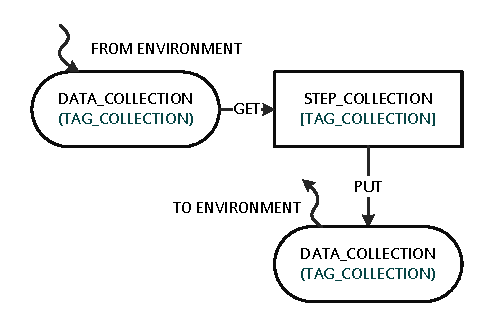
\includegraphics[width=0.5\textwidth]{drawings/CnCExample.pdf}
  \caption{CnC Graph Semantics}
  \label{fig:cnc_graph}
\end{figure}

The CnC model can be thought of as a producer-consumer paradigm where
data is produced and consumed by tasks, or ``steps'' in CnC
terminology. The produced and consumed data is declared explicitly in
an input file, known as a ``graph file''. The steps themselves are
also entities that can be produced. When a step produces another step,
this is known as a ``control dependency'' and is also declared in the
graph file.

Figure~\ref{fig:cnc_graph} shows a graph file. The rectangles are
``step collections'', the ``data collections'' are ovals, and the
dependencies are directed edges between them. The title of a step
collection is usually a descriptive verb and the title of a data
collection is usually a descriptive noun. The control dependencies are
not shown. A text description of Figure~\ref{fig:cnc_graph} (which
includes control information) is provided to CnC when designing a CnC
application.
% RRL: "designing", not "running"?
Section~\ref{sec:raytracing} shows an example of this.

By declaring all dependencies between steps and data, the specifics
regarding how the algorithm is executed is abstracted out of the
implementation. For example: It is clear what data is needed by a
given step, so if that data has not been produced yet, the step will
not be scheduled. This allows the runtime to optimally decide when and
where to schedule computation. By way of contrast, in a conventional
multithreaded program, it is the responsibility of the programmer to
guarantee that a thread's inputs are available and consequently start
the thread.

For some more complicated semantics, additional hints can be provided
to the runtime through a ``tuning specification''. As the tuning
specification usually is in a separate file, this makes it easy to run
the same program on different architectures, as no rewrites of the
application are necessary to switch platforms: just the tuning
specification.

\subsubsection{Language Specifics}
The CnC model is built on three key constructs; step collections, data
collections, and control collections ~\cite{budimlicconcurrent}. A
step collection defines computation, an instance of which consumes and
produces data. The consumed and produced data items belong to data
collections. Data items within a data collection are indexed using
item ``tags'': tuples that, like primary keys, can uniquely identify a
data item in the data collection. Finally, the control collection
describes the prescription, or creation, of step instances. The
relationship between these collections as well as the collections
themselves are defined in the graph file.

Developing a CnC application then begins with designing the graph
file. An algorithm is broken down into computation steps, instances of
which correspond to different input arguments. These steps, along with
the data collections become nodes, in the graph. Each step can
optionally consume data, produce data, and/or prescribe additional
computation. These relationships: producer, consumer, and control,
define the edges of the graph and will dynamically be satisfied as the
program executes.

The next and final required step in producing a CnC application is to
implement the step logic. The flow within a single step is: consume,
compute, and produce. This ordering is required as there is no
guarantee the data a step needs will be ready when the step begins
executing. This is due to steps being preemptively scheduled when they
are prescribed. Most of the time the data \emph{will} be ready when a
step begins execution, but occasionally and often due to an
implementation error, a step's data may never be available.
Internally, if the data is not ready when a step begins execution
it will halt execution and try again later. To improve performance,
hints can be provided through the tuning specification to increase the
likelihood that steps are schedule for execution when their required
input data is ready.

\subsection{Example}

\begin{figure}[!tb]
  \centering
  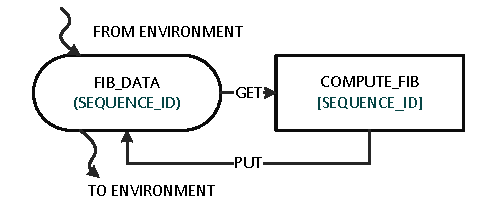
\includegraphics[width=0.5\textwidth]{drawings/FibExample.pdf}
  \caption{A CnC Graph to Compute the Fibonacci Sequence}
  \label{fig:fib_graph}
\end{figure}

% apparently putting this here makes it show up on the top of page 3, where I want it
\begin{figure*}[t]
  \centering
  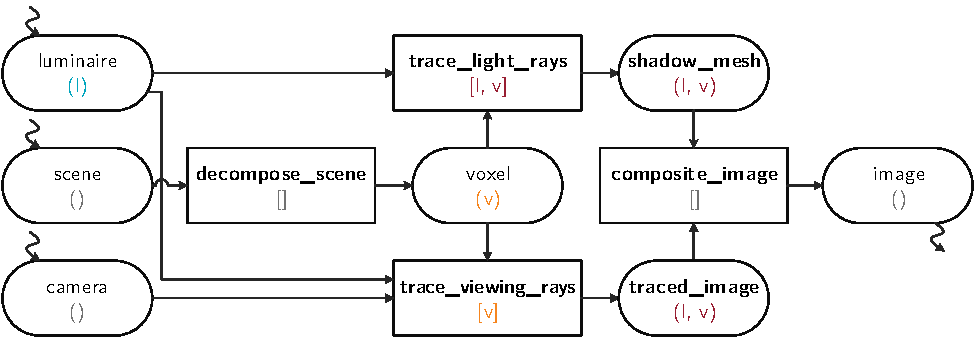
\includegraphics[width=\textwidth]{drawings/CnC.pdf}
  \caption{CnC Graph}
  \label{fig:cnc}
\end{figure*}

Figure~\ref{fig:fib_graph} shows an example of a
simple iterative implementation of the Fibonacci sequence. This
application consists of one step, COMPUTE\_FIB, which takes the
previous two computed values as input and produces the next value in
the sequence. One data collection, FIB\_DATA, exists for the
application. Data within the collection is indexed by a tag consisting
of the sequence number. Tags 1-5, then index the values 1,
1, 2, 3, 5, respectively. The first two values of the data collection
are produced by the environment, the rest of the values in the
collection are produced as needed by COMPUTE\_FIB. A tag exists for
COMPUTE\_FIB as well. We can index this collection by the integer
sequence a particular instance will produce. For example, the step
% RRL: What do you mean by "integer sequence"? The *whole* Fibo sequence?
instance at tag 3 will consume the data at tag 1 and 2, and produce
data at tag 3. Specifically it will consume 1, 1 and produce 2.
The number of steps executed in this example is provided by the 
environment.

\section{Distributed Ray Tracing}

\emph{"Ray tracing is the future and ever will be"} was the title of a SIGGRAPH 
course in 2013.  The course outlined the state of the art in ray tracing 
technology, covering recent developments and optimization techniques to speed up 
the core algorithm such as acceleration data structures.  This quote points out 
that although we have optimized ray tracing to a T, it is still not the primary
rendering technique used in graphics.  This section outlines key strategies for 
ray tracing optimization with an emphasis on parallel and distributed 
advancements.

Ray tracing is an application that tends to scale well as you subdivide the 
task.  Each ray cast into a scene does not need any information about any other 
ray cast into the scene.  Communication between rays, therefore, is non-existent 
and only the cost of creating new tasks and joining the tasks to produce the 
final ray traced image limit the amount of parallelism you can extract from the
algorithm\footnote{ %
  The system you are executing a ray tracer on limits the parallelism of the 
  application more than the algorithm.  
}.

Although no ray depends on any other ray in a ray tracing algorithm, the data 
needed by each individual ray varies widely as its path is traced. Acceleration 
structures such as k-d trees have been developed to increase ray tracing 
performance. As the size of the scene increases, however, it is no longer 
possible to store an entire data set in an acceleration structure in shared 
memory.

One solution is to implement data decomposition. Each node on a distributed 
system is then responsible for a subset of the domain. Primary, secondary, 
and subsequent rays are then communicated across nodes as the algorithm 
executes. These types of models typically rely on expensive pre-processing steps 
that help to balance both the data distribution and rendering work evenly across 
nodes ~\cite{navratil2014dynamic}.

Load balancing, a significant bottleneck on today's systems, may not be easily 
implemented on exascale systems. The proposed smarter programming models and 
runtimes, on the other hand, will allow for scheduling and data movement 
decisions to be made at runtime which will help reduce imbalance in a system. 
Data and computation can be dynamically migrated off of overworked nodes 
(assuming a properly sized granularity for tasks and data).

%%% Local Variables: 
%%% mode: latex
%%% TeX-master: "main"
%%% End: 
 % subsections: distributed ray tracing, task-based
                          % programming models, cnc model, petri net

\chapter{Design}
\label{sec:design}

Libraries such as Embree, see section~\ref{sec:embree}, provide optimized ray 
tracing algorithms that exploit parallelism on a single machine.  When we look
at larger data sets that will no longer fit into the memory of a single machine,
we may consider the use of distributed systems, see section~\ref{sec:computing},
to render images.  The next generation of distributed systems capable of 
exascale computation provides an opportunity and in some cases a necessity to 
redesign current distributed applications.  Two of the main differences that 
will set exascale systems apart from current distributed systems are the 
increase in the number of nodes available and the reduction of the memory 
available per node.  For algorithm designers, this means there will be increased
communication overhead as data will need to be passed more frequently between 
individual nodes.

Communication avoiding algorithms have been proposed as a way to reduce 
communication overhead.  The basic idea is to re-do computation when possible
instead of communicating results.  We use this idea as a basis for designing a 
distributed ray tracing application.  On node parallelism can be exploited by
taking advantage of Embree or another optimized library.  This leaves the key 
challenge as how to reduce the communication necessary between the nodes of the 
distributed system.

\section{Data Decomposition}
\label{sec:data_decomposition}
Designing a ray tracer for exascale systems becomes an interesting problem once
we consider scenes to render that have too much information to fit entirely into
the memory of a single node.  In these scenes, some type of data decomposition 
is required where the scene is divided into smaller pieces and distributed 
amongst the available nodes. To fully utilize the on node parallelism we would 
want to give each node enough data to fill its available memory. As each scene 
to be rendered is unique the idealized distribution for one scene will not be 
the same as the idealized distribution for another.  This introduces the concept 
of load balancing.

Load balancing is often addressed with a pre-processing step where the domain is 
optimally divided into evenly sized chunks of data before ray tracing beings. 
As the pre-processing step is often computationally expensive, the expense must 
be considered and weighed against alternative designs. For example, a naive 
alternative approach is to divide the space based on a uniform spatial 
distribution.  This results in unevenly balanced chunks of data but takes little
time to compute.  In this naive approach where the scene has not been balanced 
it is likely to end up with nodes that have lots of work while other nodes have 
little work.

Determining the optimal design pattern for data decomposition becomes a question
of whether the cost of pre-processing outweighs the cost of an unbalanced 
system.  Assuming the pre-processing step were free, computationally speaking, 
the solution would then be to use it.  This would ensure the minimum number of
nodes are used and that each one is used to its full potential, memory wise.  
However since there is a cost to pre-processing we must consider algorithms that
reduce this cost.  

Dividing the domain uniformly in space for example reduces the pre-processing 
cost but requires the use of more nodes then would be needed by a load balanced
distribution.  In addition, each node may or may not fill the memory available. 
Since each node need not be responsible for a single chunk of the domain, it is 
possible of offset this concern and increase memory usage per node by assigning 
each node multiple chunks of data.

\begin{figure}[!htb]
\centering
  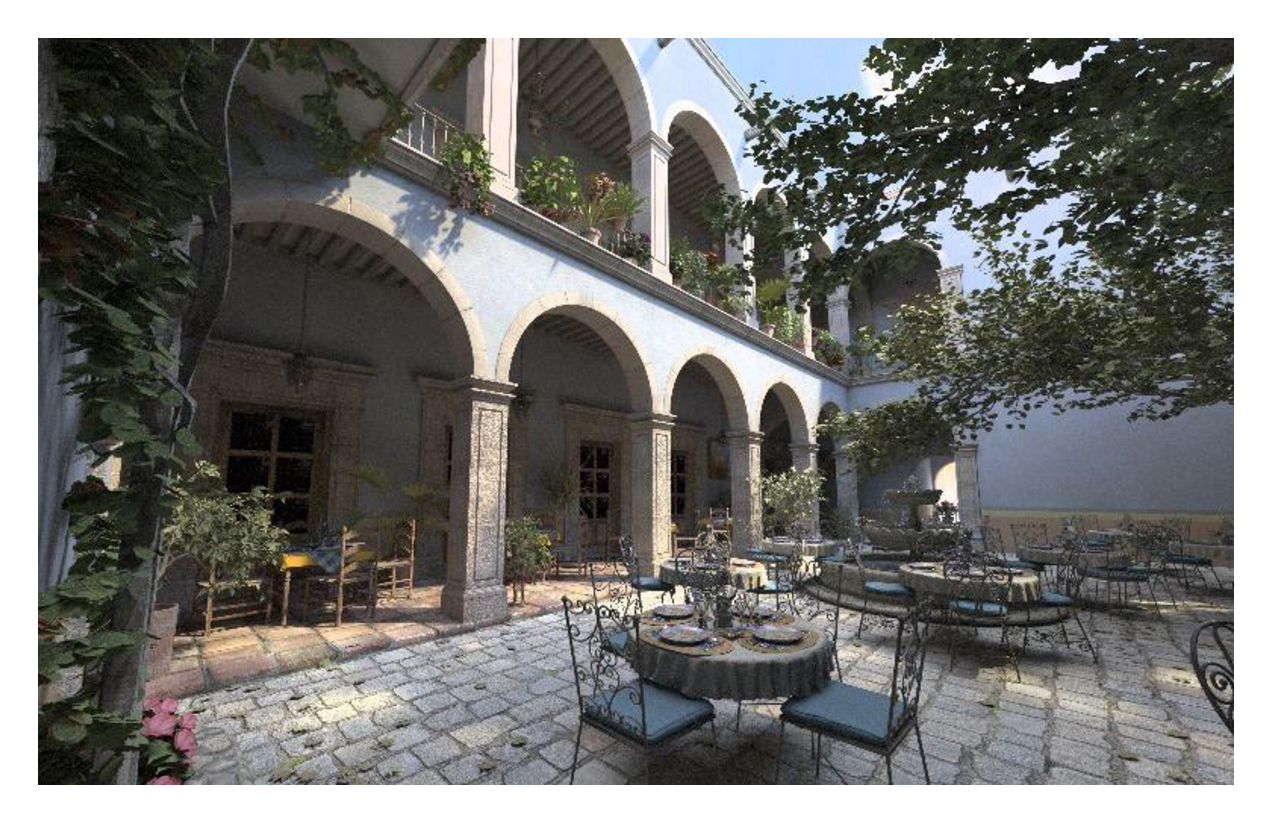
\includegraphics[height=5cm]{drawings/sanmiguel_cam25.pdf}
  %\footnote{
  %\href{http://www.pbrt.org/scenes_images/sanmiguel\_cam25.jpg}
  %               {http://www.pbrt.org/scenes_images/sanmiguel\_cam25.jpg}}
\caption{San Miguel example scene}
\label{fig:san_miguel}
\end{figure}

As an example we will consider the San Miguel data set, see 
Figure~\ref{fig:san_miguel}.  The scene was modeled by Guillermo M. Leal Llaguno
and is based on San Miguel de Allendo, Mexico.  It is a large scene with a 
nonuniform data distribution.  If we decompose the domain into twenty-seven 
spatially equal parts, we get the distribution shown in 
Figure~\ref{fig:san_miguel_data} a.  If we consider ray tracing this scene on a
machine with eight cores, we might get a distribution such as that shown
in Figure~\ref{fig:san_miguel_data} b.   This roughly distributes the data 
evenly between the nodes and positions neighbors on the same cores, giving us a
setup similar to what a pre-processing step designed to optimally distribute the 
data may compute.  For simplicity we will use the spatially uniform data 
distribution algorithm and focus on reducing communication cost.

\begin{figure}[!htb]
\minipage{0.52\textwidth}
  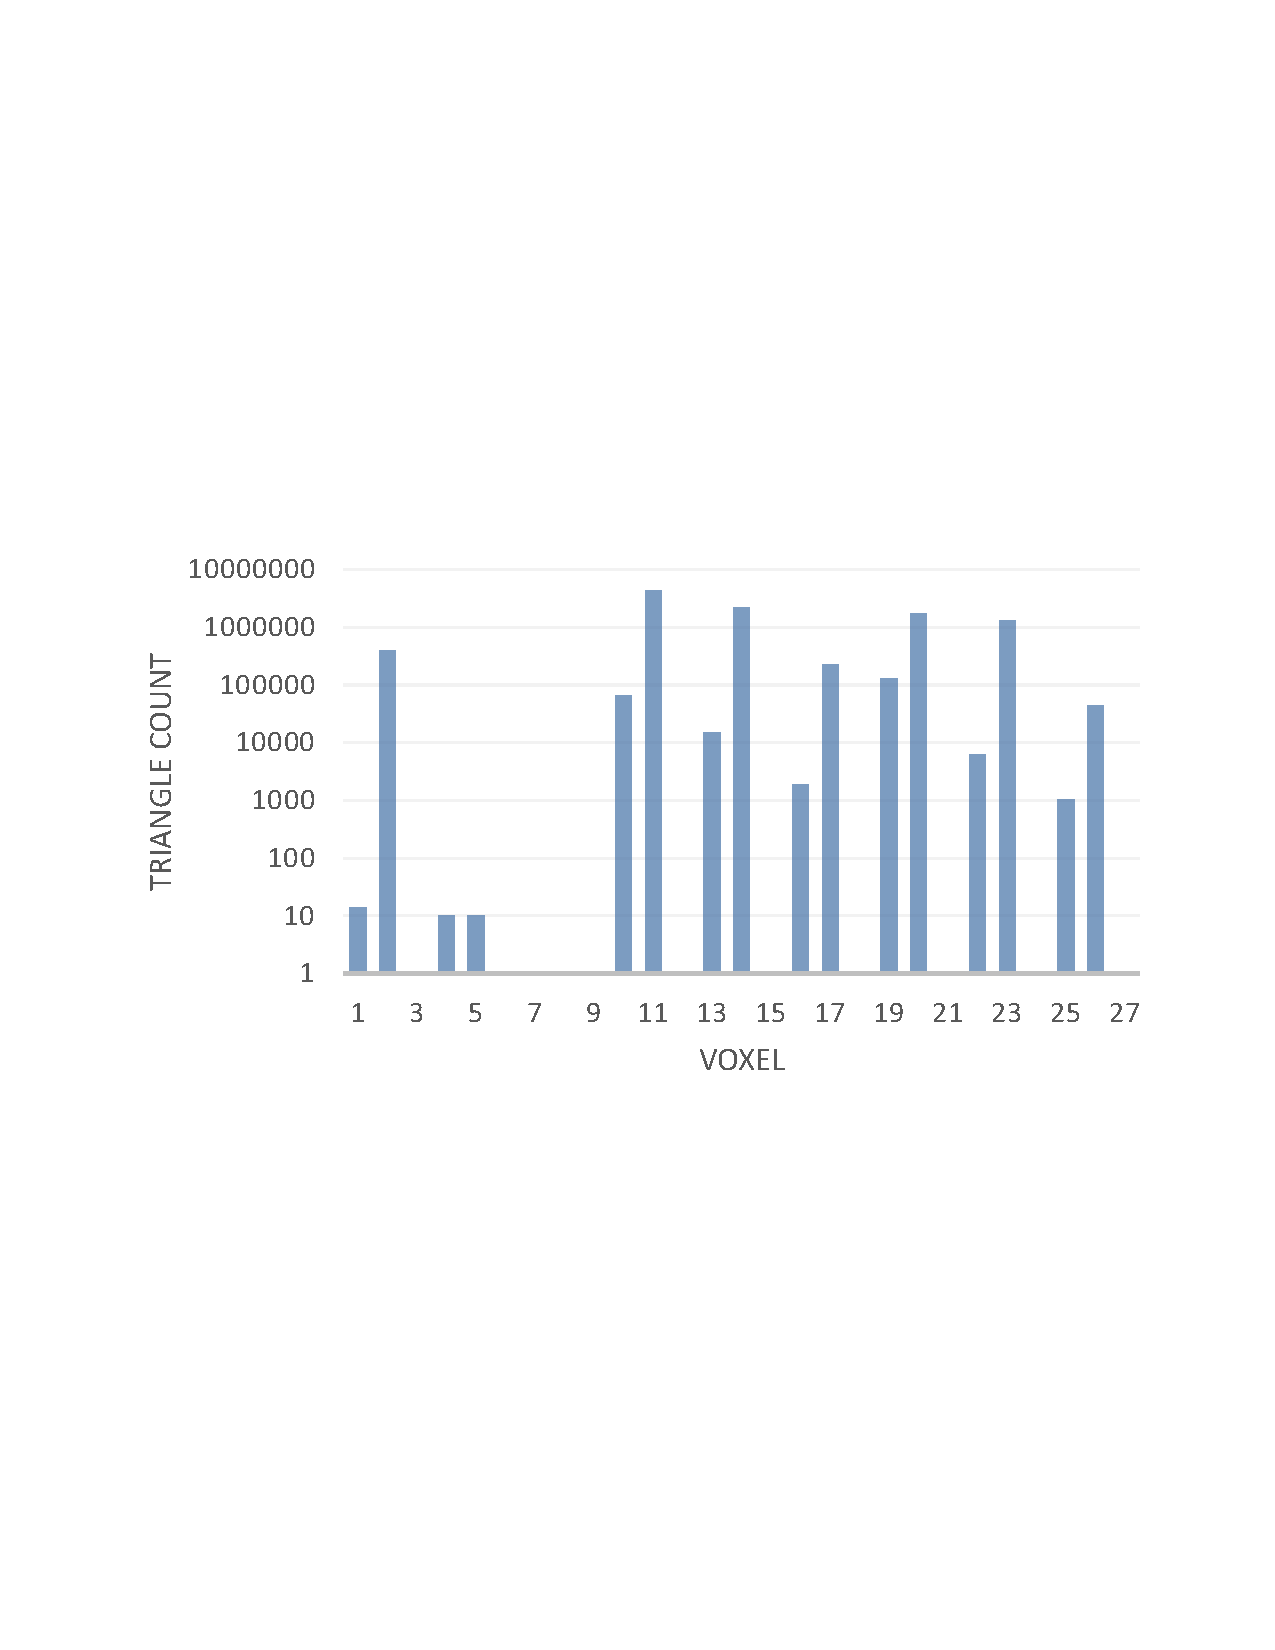
\includegraphics[height=3.8cm]{drawings/VoxelDistribution.pdf}
  
  (a) Triangles per voxel
  
  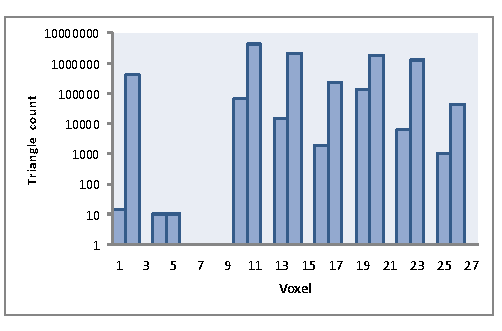
\includegraphics[height=3.8cm]{drawings/DataDistribution.pdf}
  
  (c) Triangles per node  
\endminipage\hfill
\minipage{0.48\textwidth}
  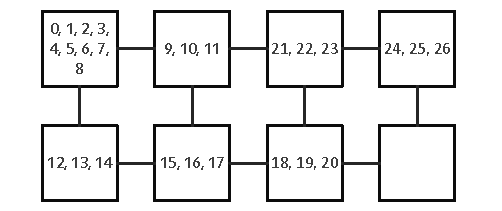
\includegraphics[width=\linewidth]{drawings/NodeDistribution.pdf}  
  
  (b) Node distribution  
\endminipage
\caption{San Miguel data decomposition example}
\label{fig:san_miguel_data}
\end{figure}


\section{Communication} 
\label{sec:communication}
Each ray cast into a scene has the potential to interact with every triangle in
the scene due to reflection and refraction\footnote{ %
  Typically a maximum threshold is set to limit the number of times a ray
  can be reflected. 
}.  In addition each point being illuminated within a scene needs to cast 
secondary rays towards the lights.  These means determining which pieces of 
memory each ray will need throughout the ray tracing algorithm is not a straight
forward task.  With a distributed system and in a worst case scenario, each ray 
may need to communicate with every node.  

Communication is anticipated to be the bottleneck on an exascale system which
makes reducing communication cost high priority in our algorithm design.  
Optimally our goal is to create a ray tracing algorithm with distributed data 
that needs little to no communication.  We explore how we might design a 
communication avoiding ray tracer in this section.

\subsection{Communication avoiding ray casting}
\label{sec:ca-ray-casting}
To design a communication avoiding ray tracer we will start with a simple ray
casting algorithm where only the primary viewing rays are traced. These rays are 
cast into a scene from the eye position.  If they intersect with an object, the 
ambient color is computed.  Without reflection, refraction and secondary rays,
communication between nodes executing the ray tracer can be avoided entirely.

\begin{figure}[!htb]
\minipage{0.4\textwidth}
\begin{algorithm}
TRACE_RAYS(voxels) 
  in: proces for each voxel of 
      data, sorted back to front
  out: image, a ray traced scene
  rays = COMPUTE_PRIMARY_RAYS
  for all voxel in voxels do
  rays_ = COPY(rays)
    voxel.TRACE_RAYS(rays_)
    for all ray in rays_ do
      if(ray.color) then
        image[ray.x][ray.y].color
         = ray.color;
      end if
    end for
  end for
return image
\end{algorithm}

(a) Controller code

\endminipage\hfill
\minipage{0.4\textwidth}
\begin{algorithm}
TRACE_RAYS(rays)
  in:  all primary rays
  out: all primary rays with 
       computed color
  for all ray in rays do
    if ray intersects scene then
      ray.color = COMPUTE_COLOR(ray)
    else
      ray.color = FALSE
    end if
  end for
return rays



.
\end{algorithm}

(b) Per voxel code

\endminipage\hfill
\caption{Ray casting pseudo code}
\label{fig:ray_caster}
\end{figure}

We can avoid all communication between nodes in a ray casting algorithm by 
preemptively sending every ray to every node, see Figure~\ref{fig:ray_caster} a.  
Each process executing over a chunk of data will receive every viewing ray, see 
Figure~\ref{fig:ray_caster} b.  Each process then traces the rays and computes a
color if the ray intersected an object within its data.  

\begin{figure}[!htb]
\minipage{0.5\textwidth}
  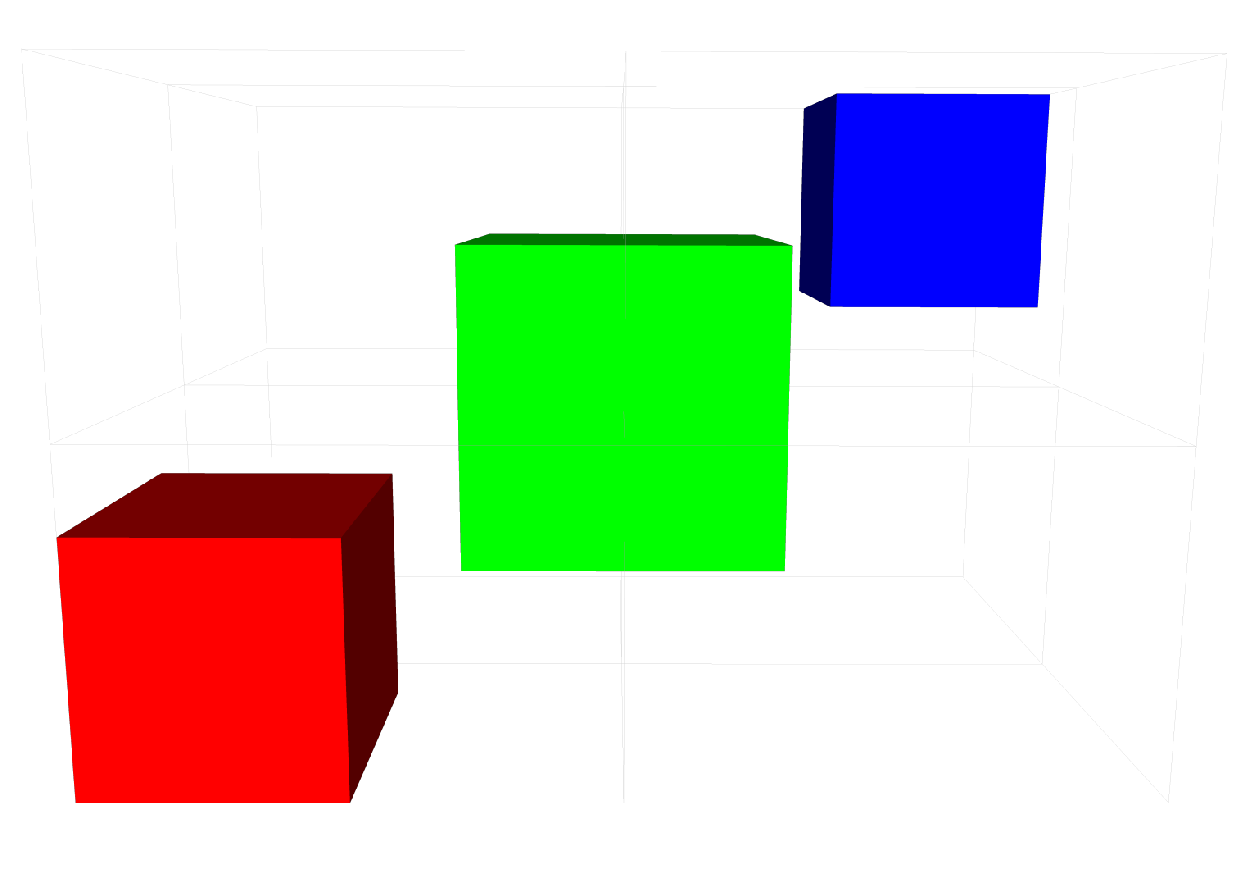
\includegraphics[width=\linewidth]{drawings/side.pdf}
  
(a) Side

\endminipage\hfill
\minipage{0.5\textwidth}
  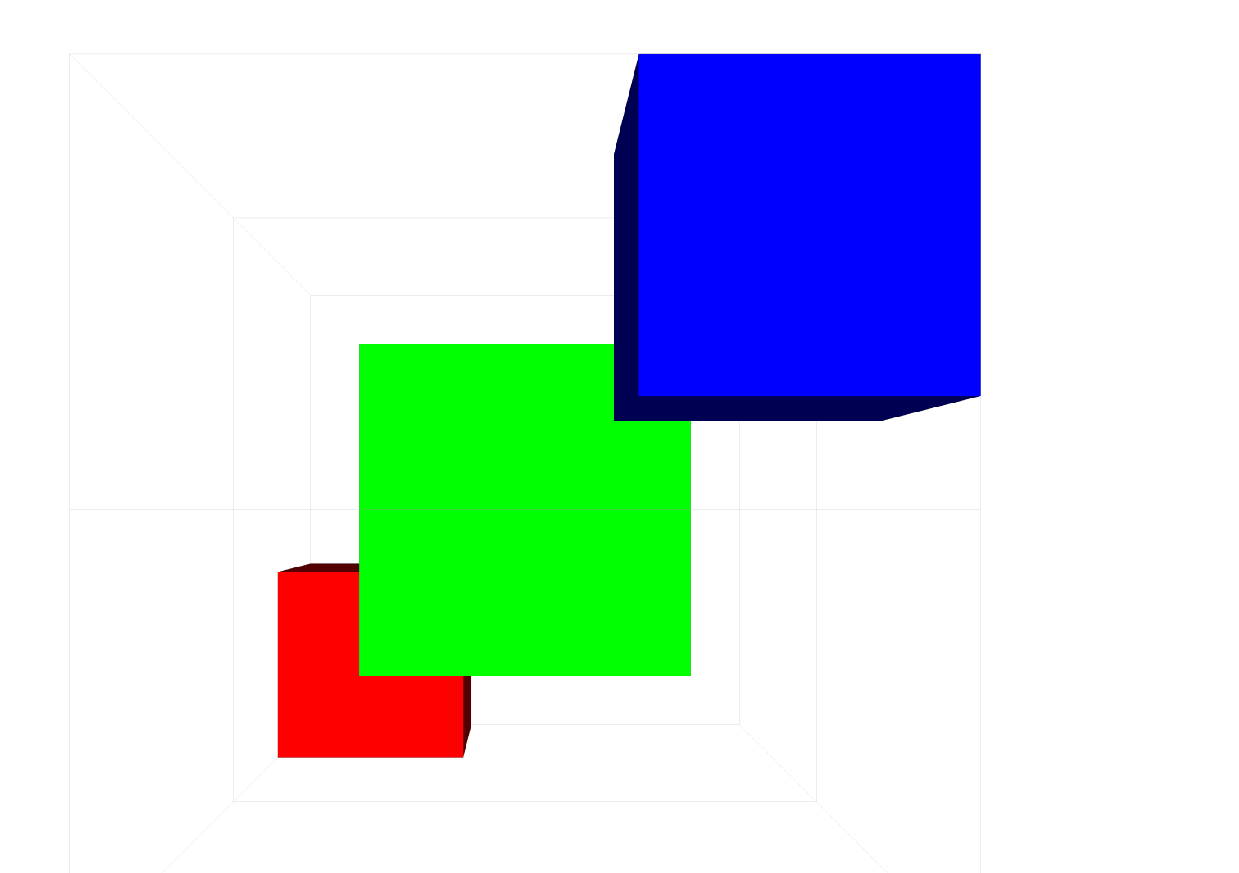
\includegraphics[width=\linewidth]{drawings/front.pdf}
  
(b) Front

\endminipage\hfill
\caption{3D view of example cubes}
\label{fig:cubes_3d}
\end{figure}

The traced rays can then be used to produce the final image using a back to 
front ordering to ensure correct image composition.  As an illustration we can 
consider a simple scene with three cubes placed along a diagonal, 
see Figure~\ref{fig:cubes_3d}.  Each cube is broken into twelve triangles, two 
for each face.  If we distribute the data into eight spatially equal pieces and 
trace the scene from the camera view shown in Figure~\ref{fig:cubes_3d} b, we 
will get the eight images shown in Figure~\ref{fig:cubes}.  These eight images 
can then be composed back to to produce into the final image, see
Figure~\ref{fig:cubes_final}.

\begin{figure}[!htb]
\minipage{0.25\textwidth}
  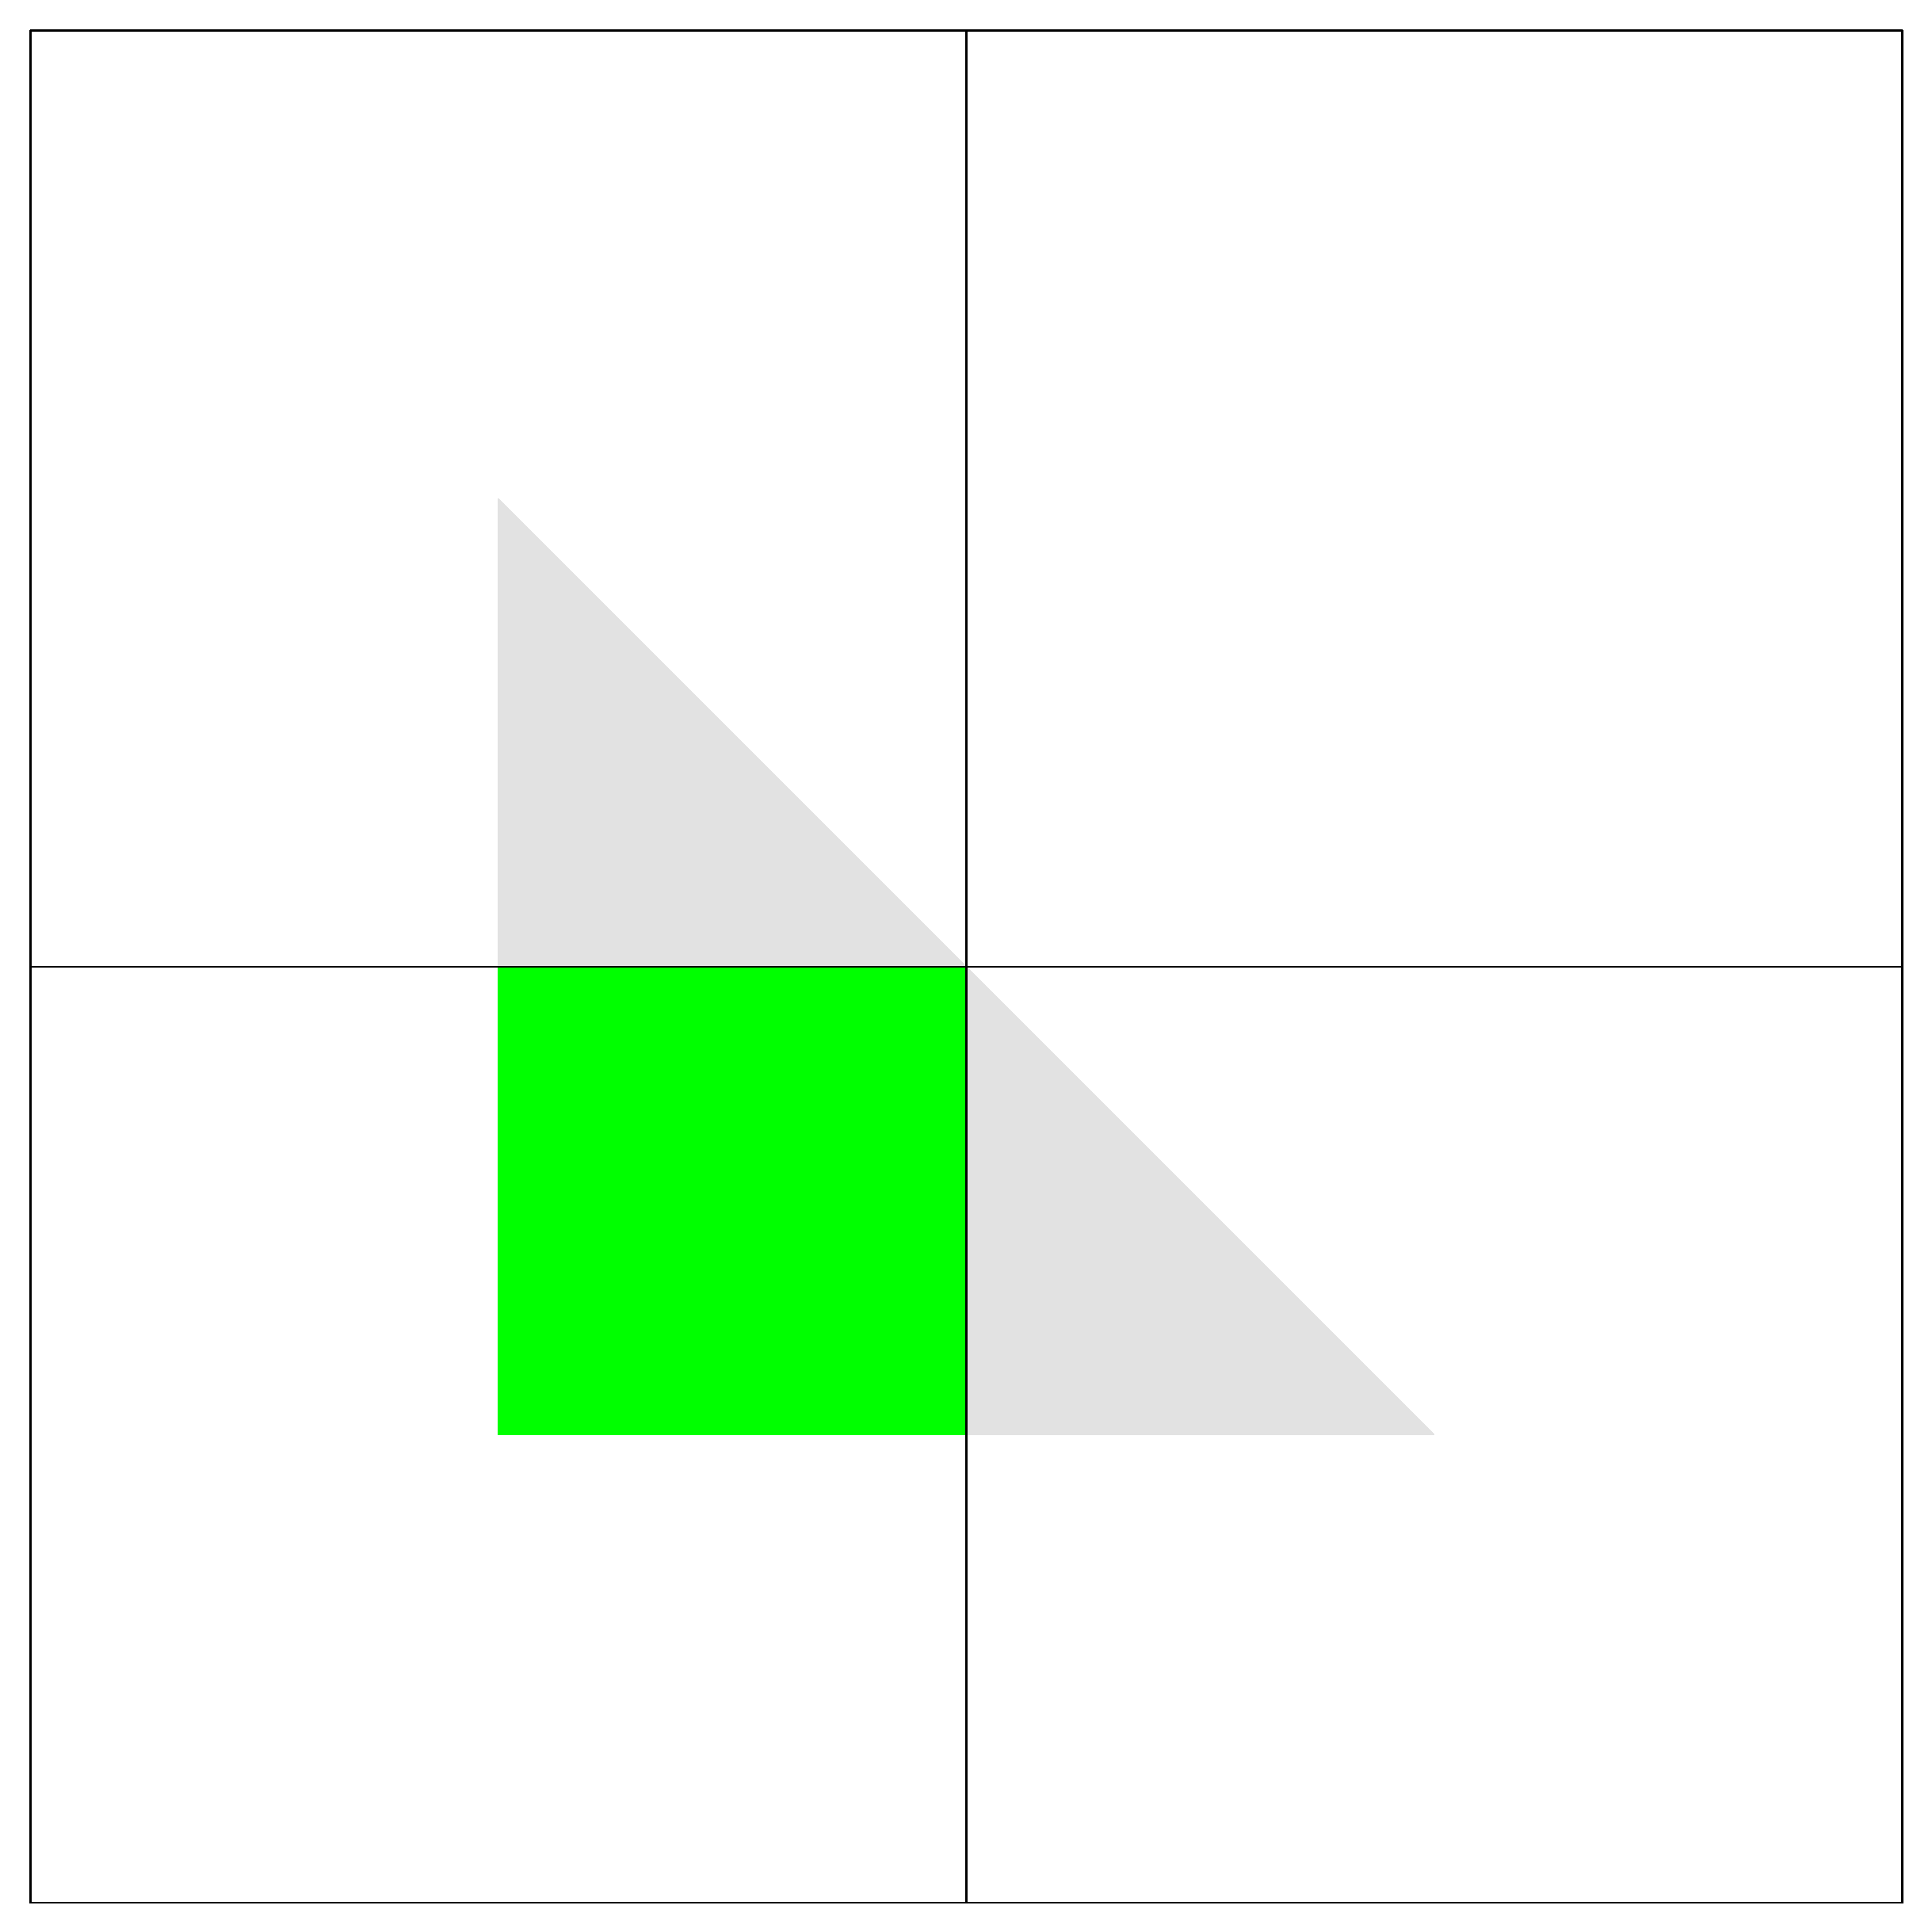
\includegraphics[width=\linewidth]{drawings/cubes_01.pdf}
  Voxel 1 
  
  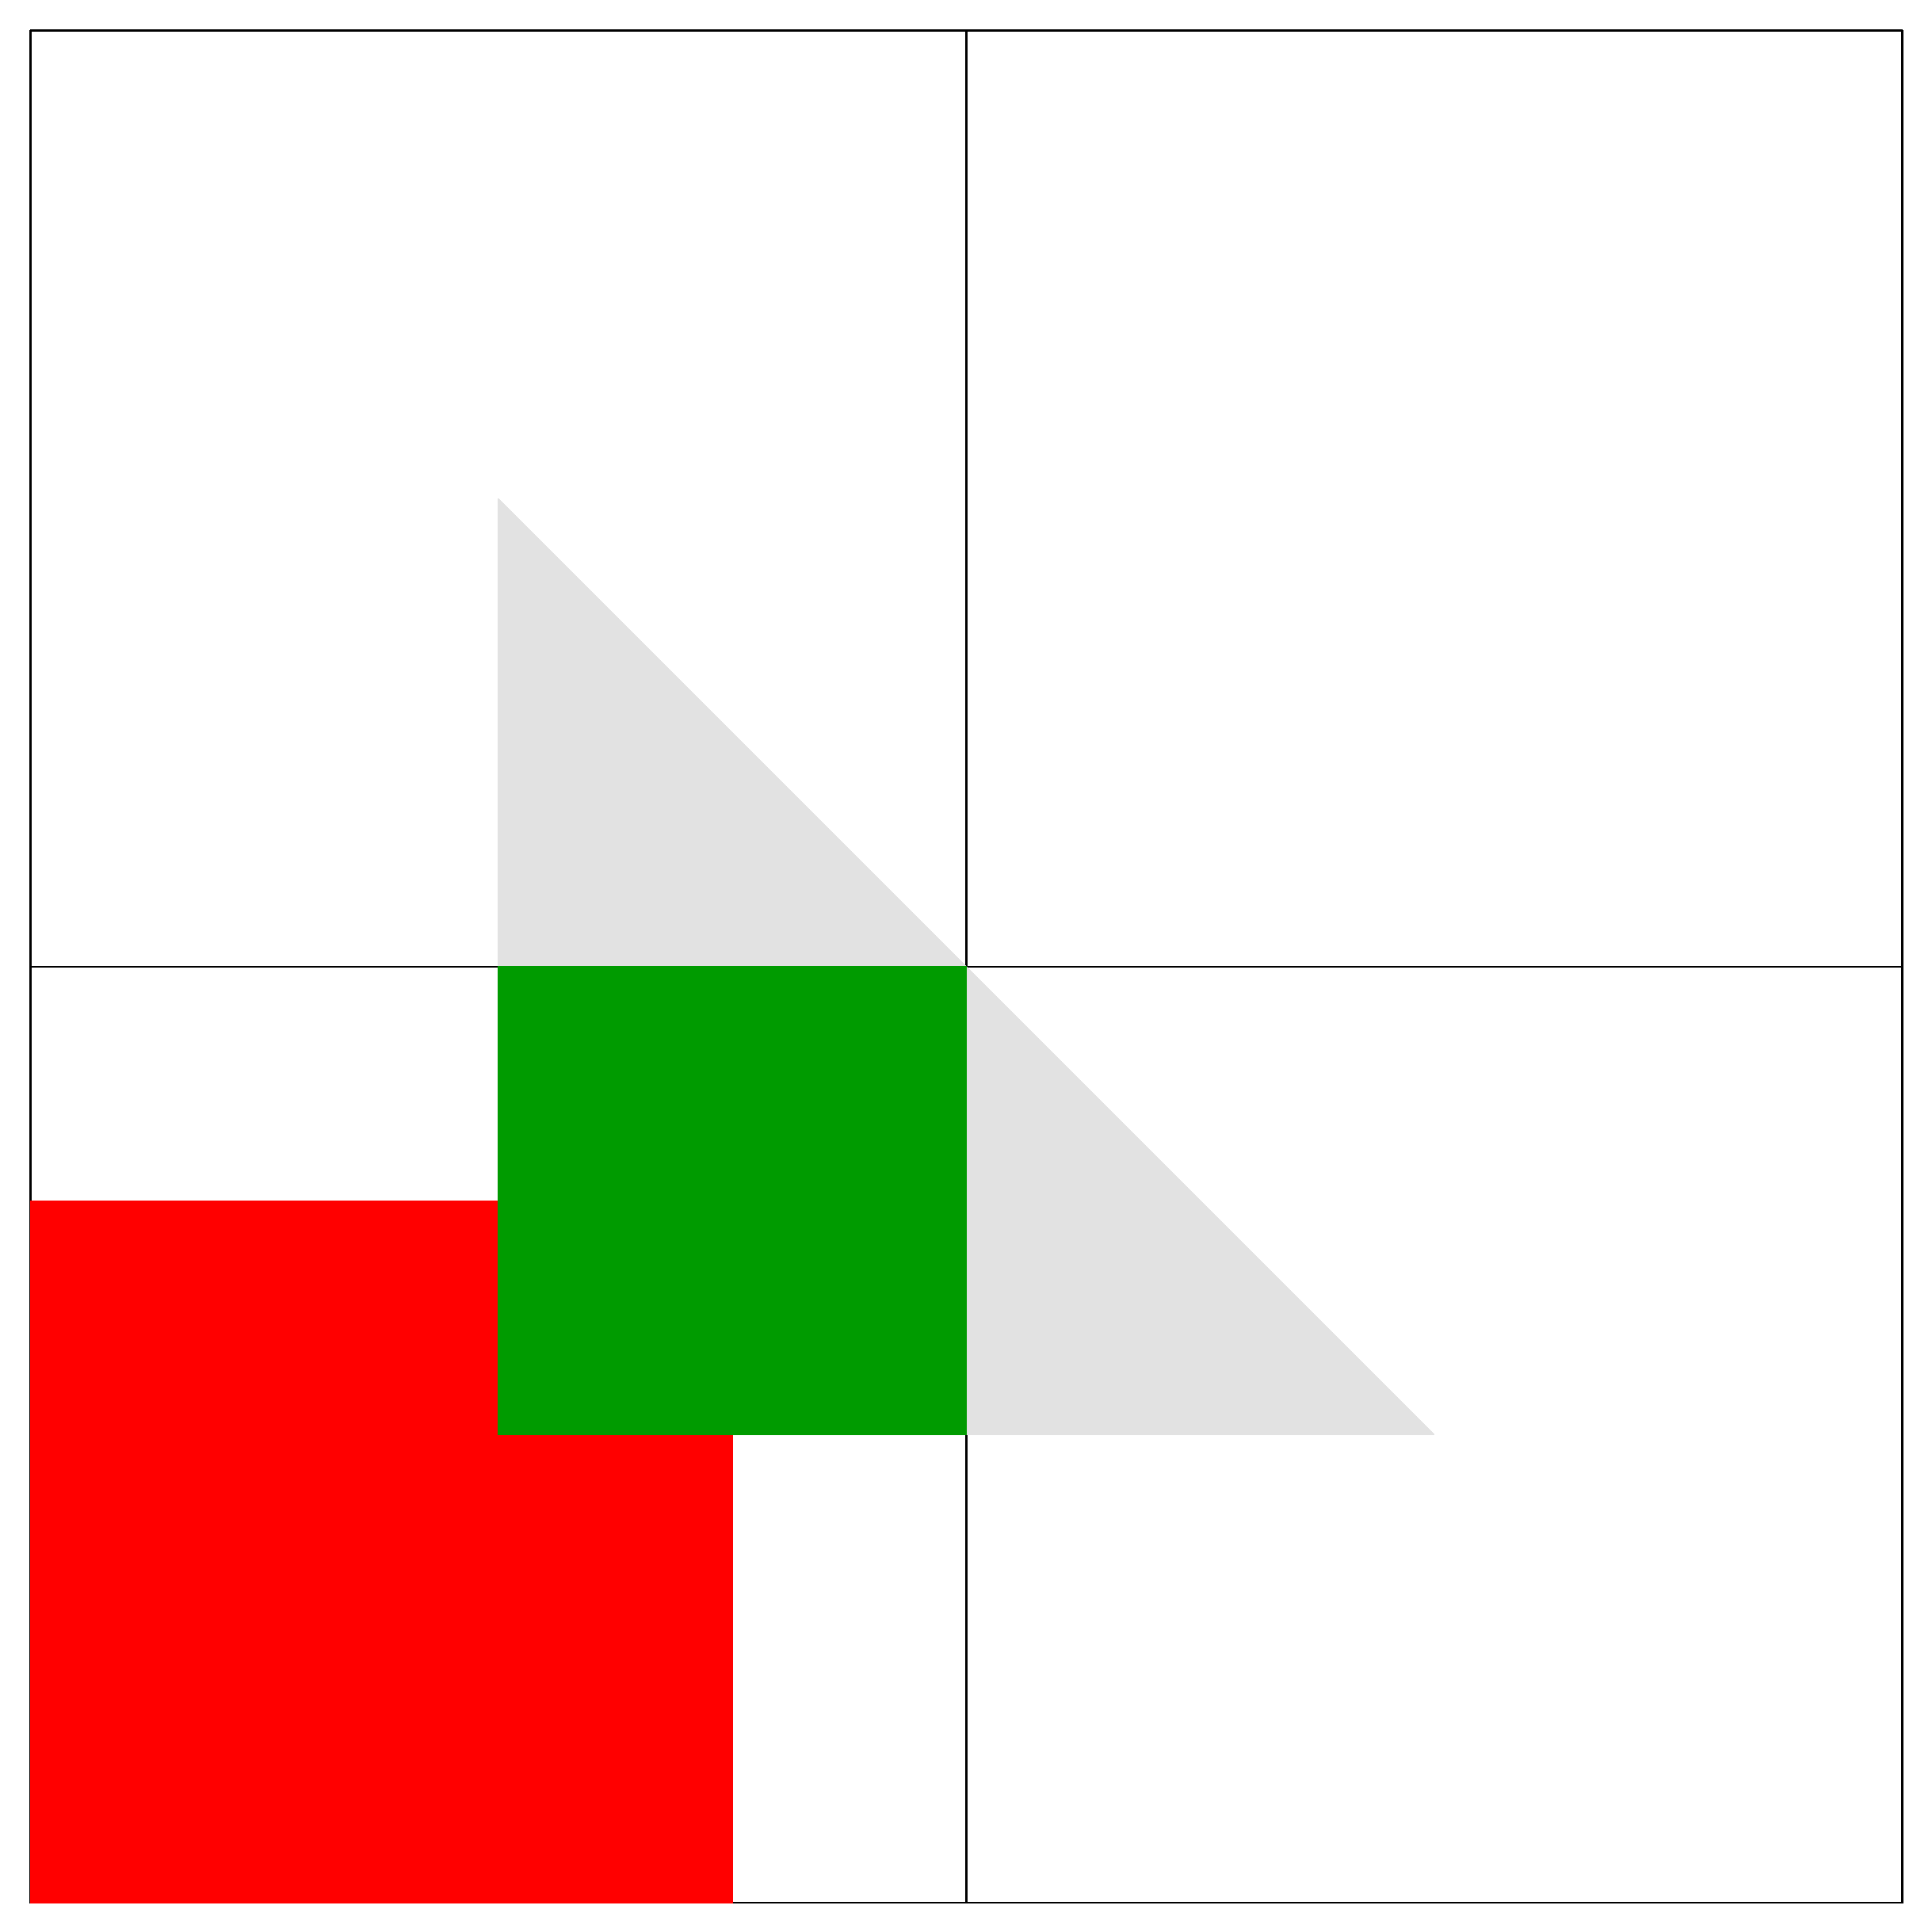
\includegraphics[width=\linewidth]{drawings/cubes_05.pdf}
  Voxel 5
\endminipage\hfill
\minipage{0.25\textwidth}
  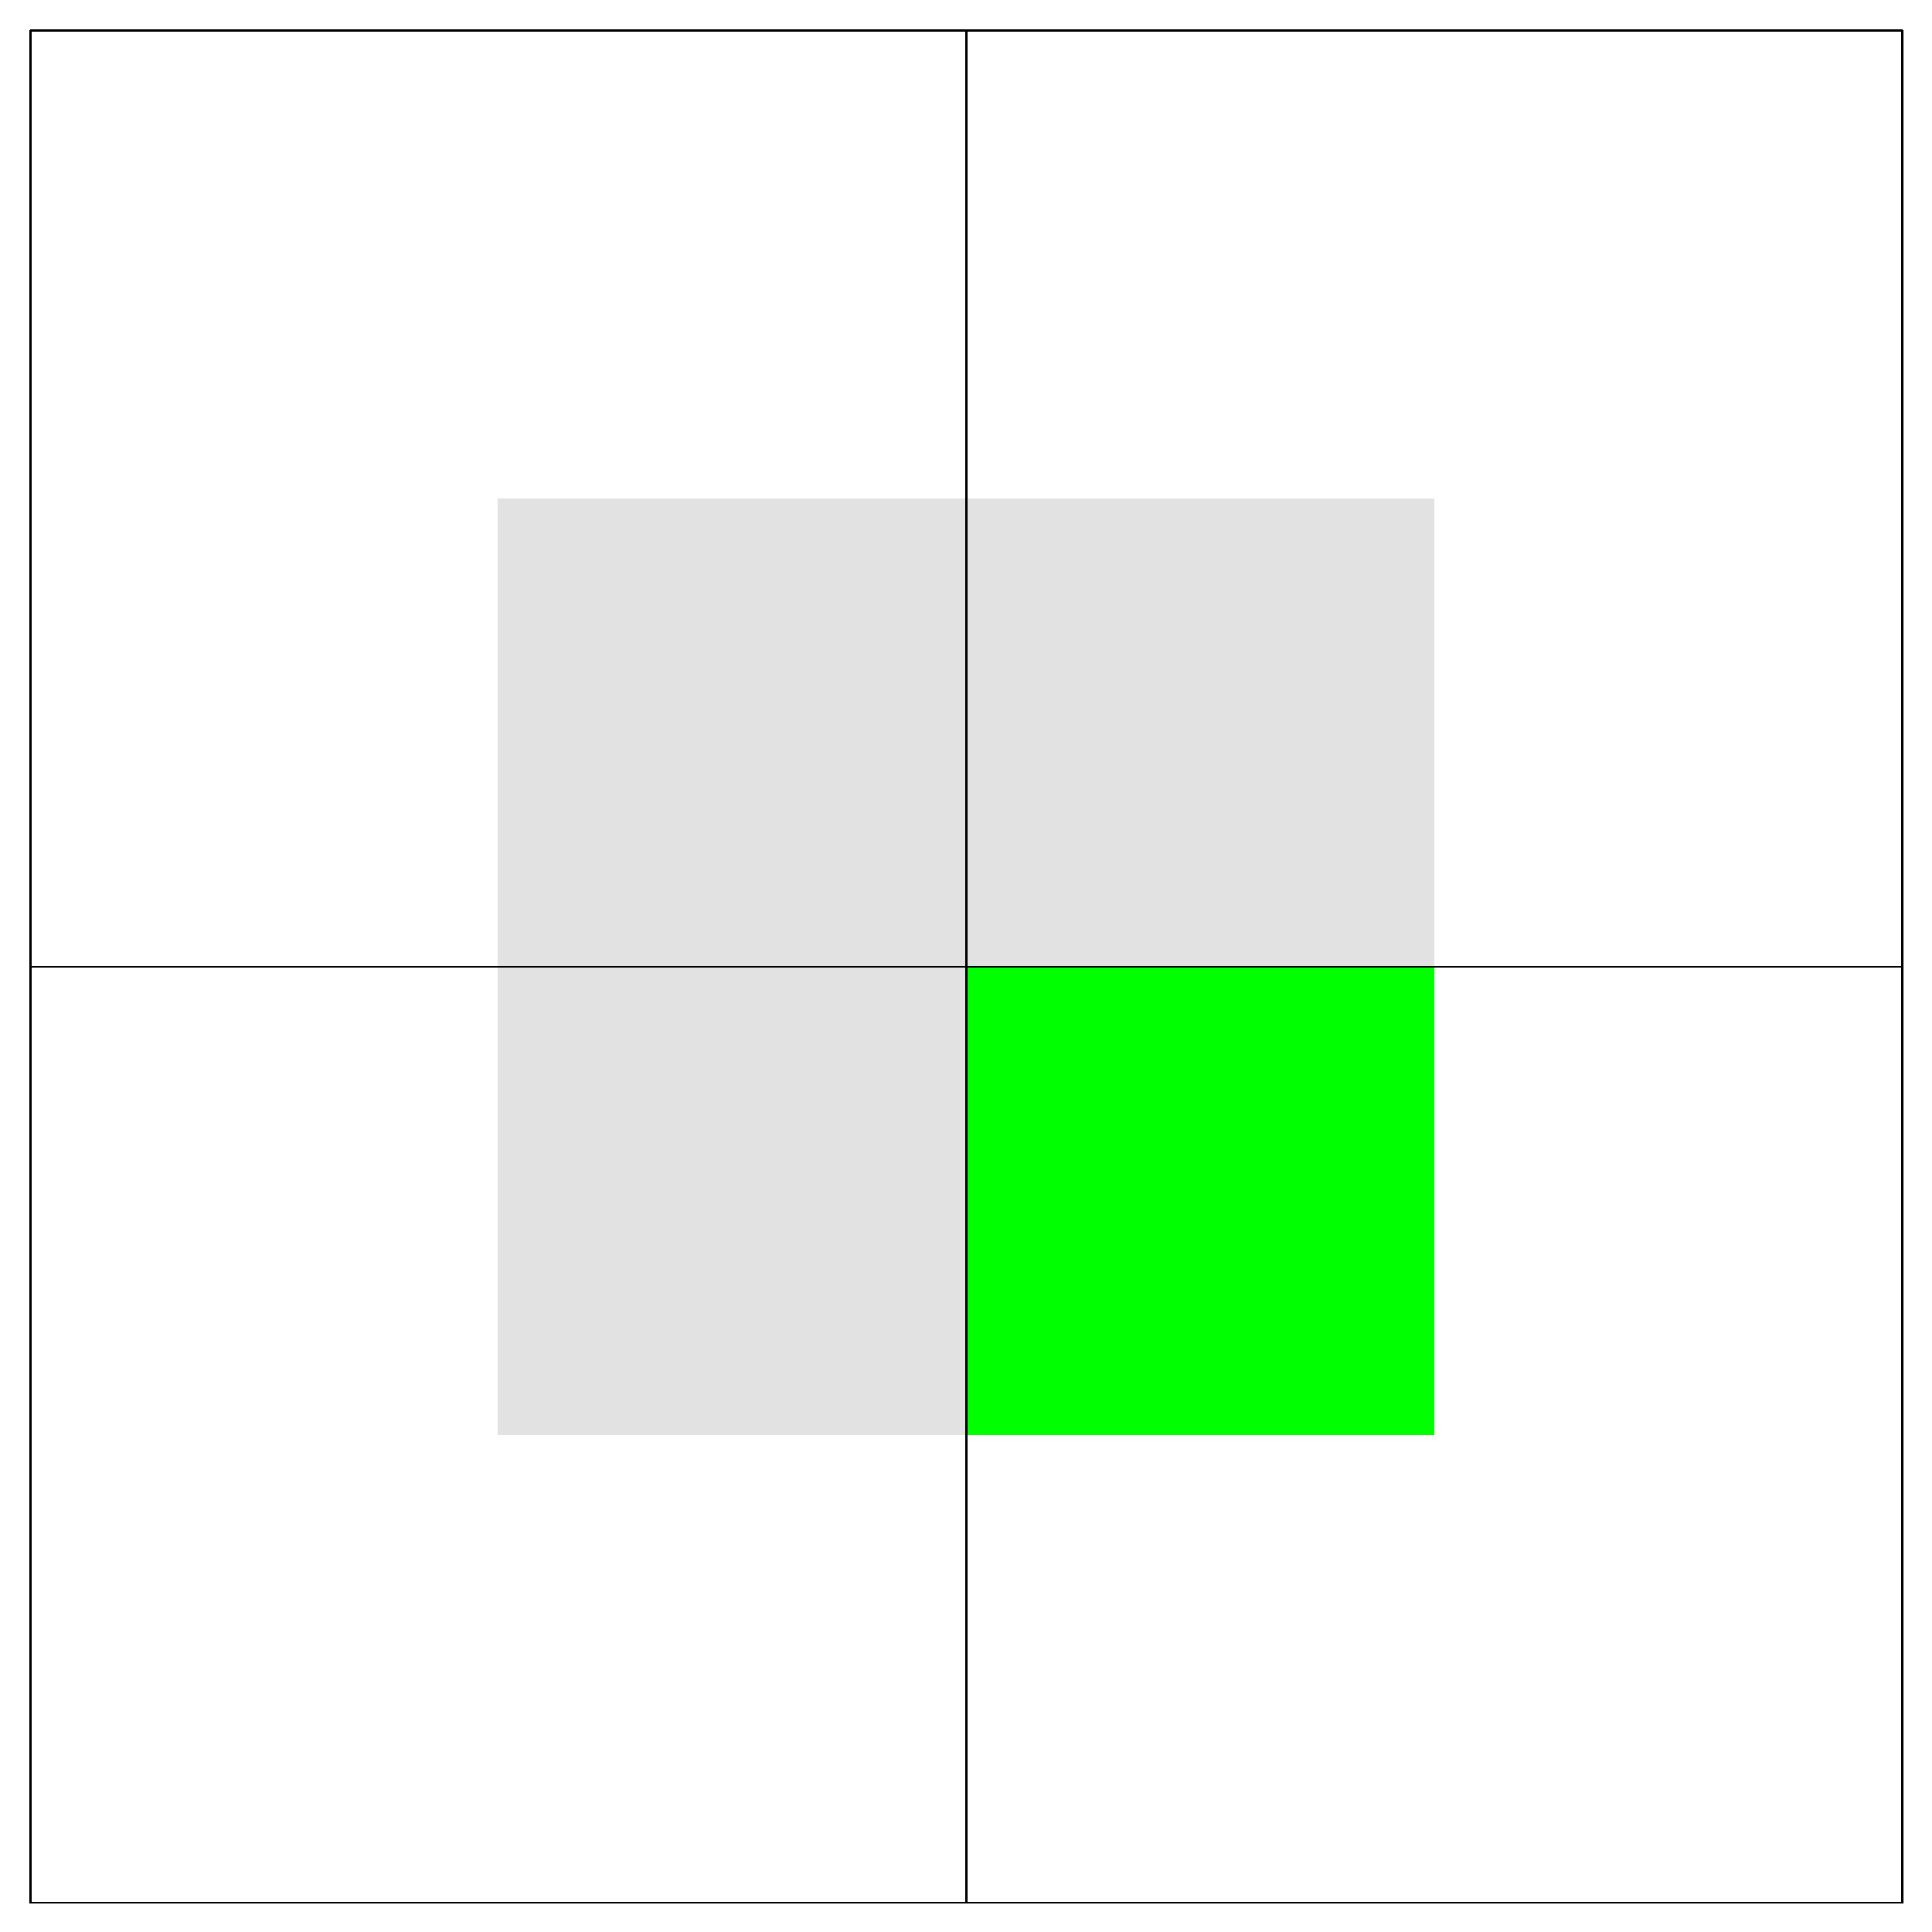
\includegraphics[width=\linewidth]{drawings/cubes_02.pdf}
  Voxel 2
  
  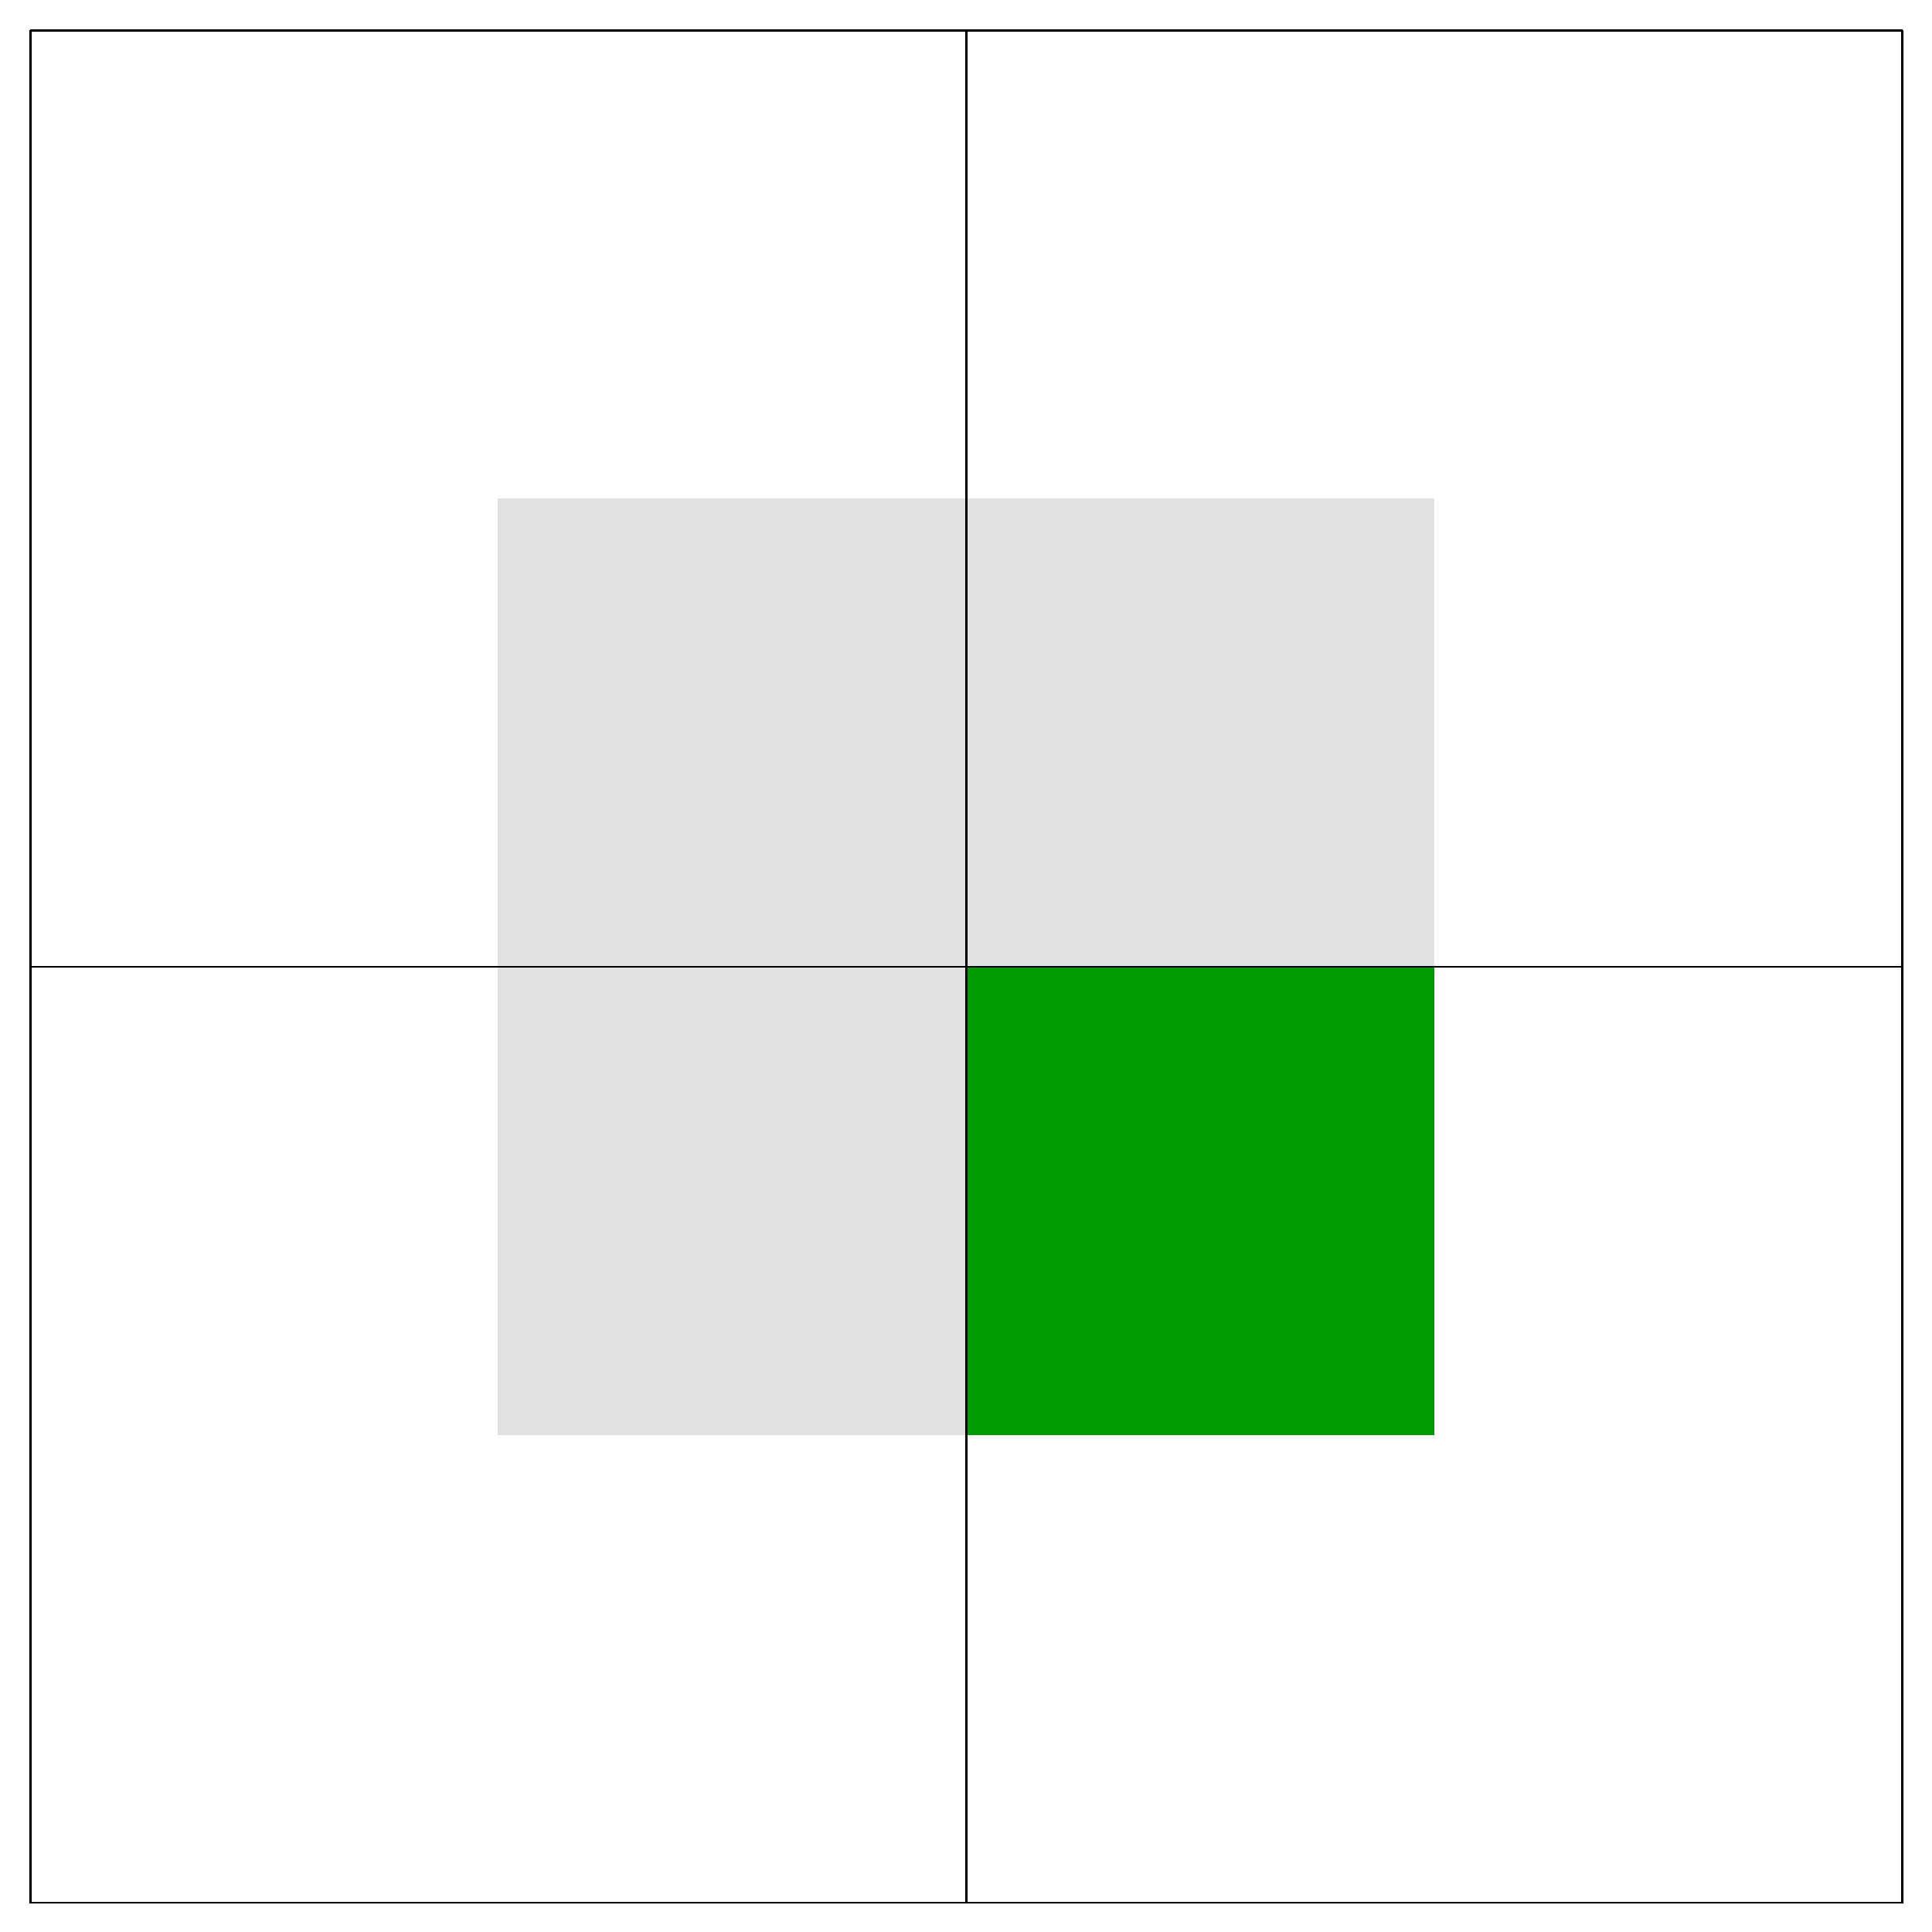
\includegraphics[width=\linewidth]{drawings/cubes_06.pdf}
  Voxel 6
\endminipage\hfill
\minipage{0.25\textwidth}%
  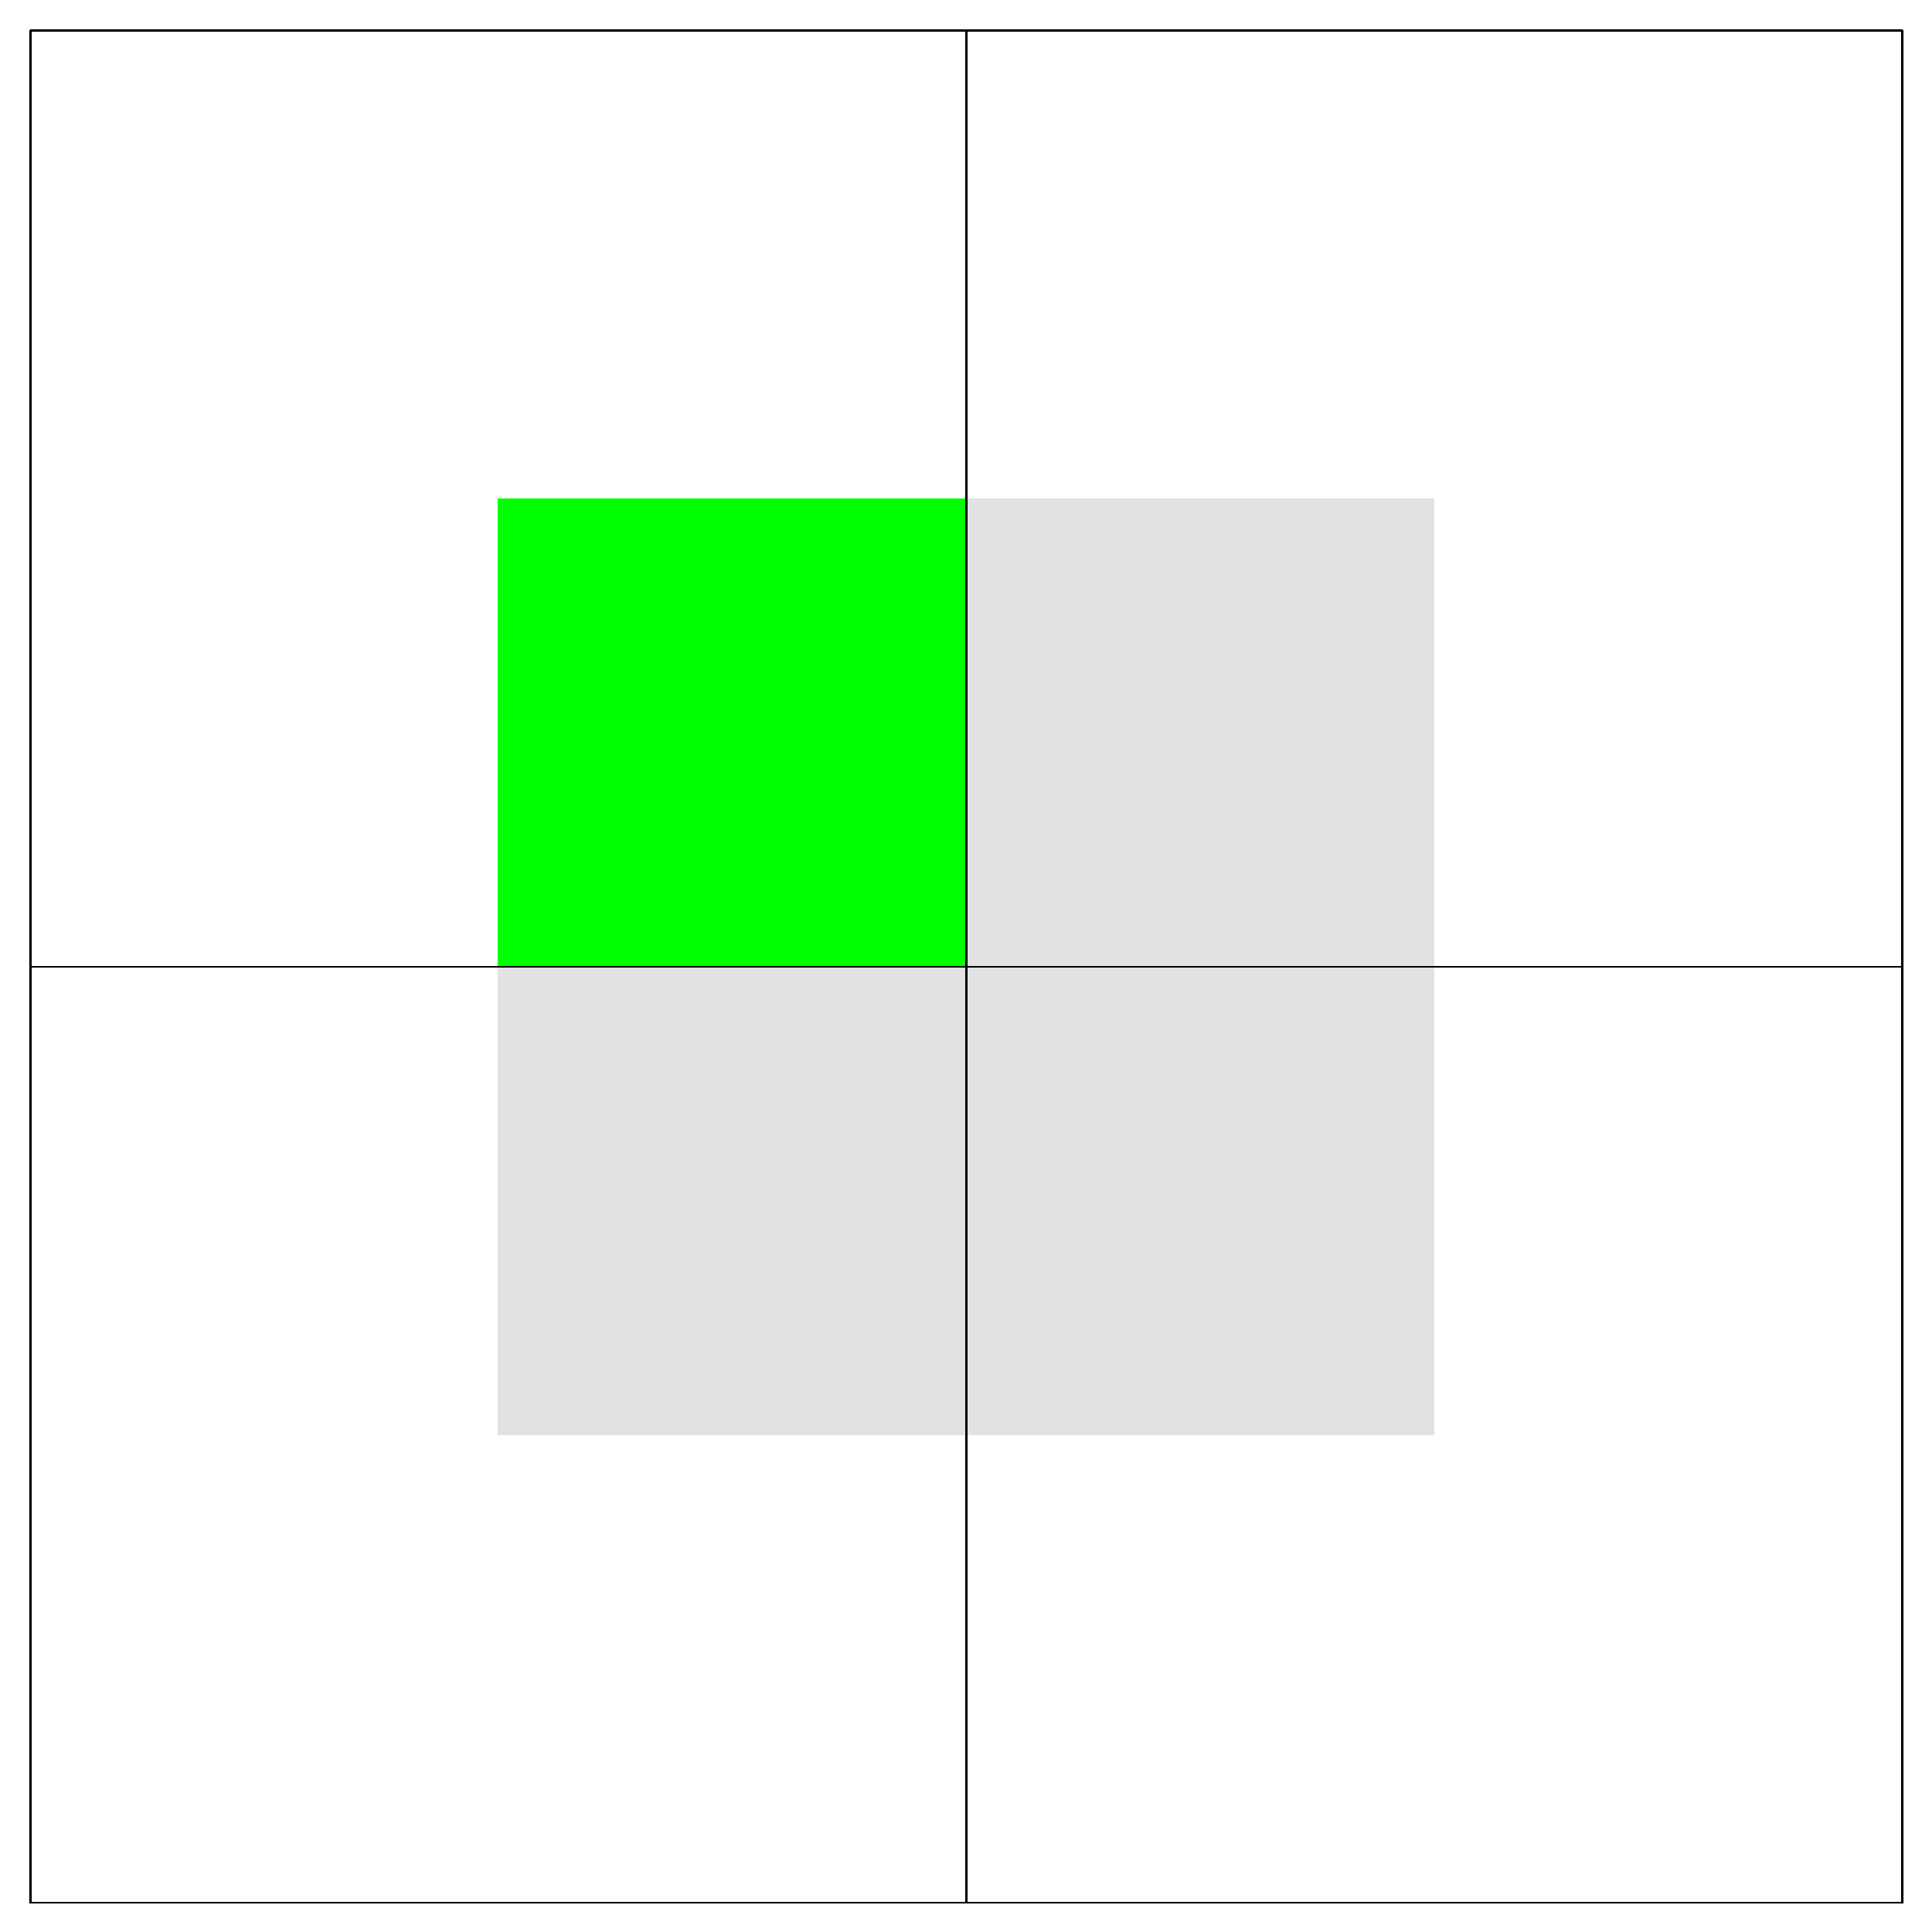
\includegraphics[width=\linewidth]{drawings/cubes_03.pdf}
  Voxel 3
  
  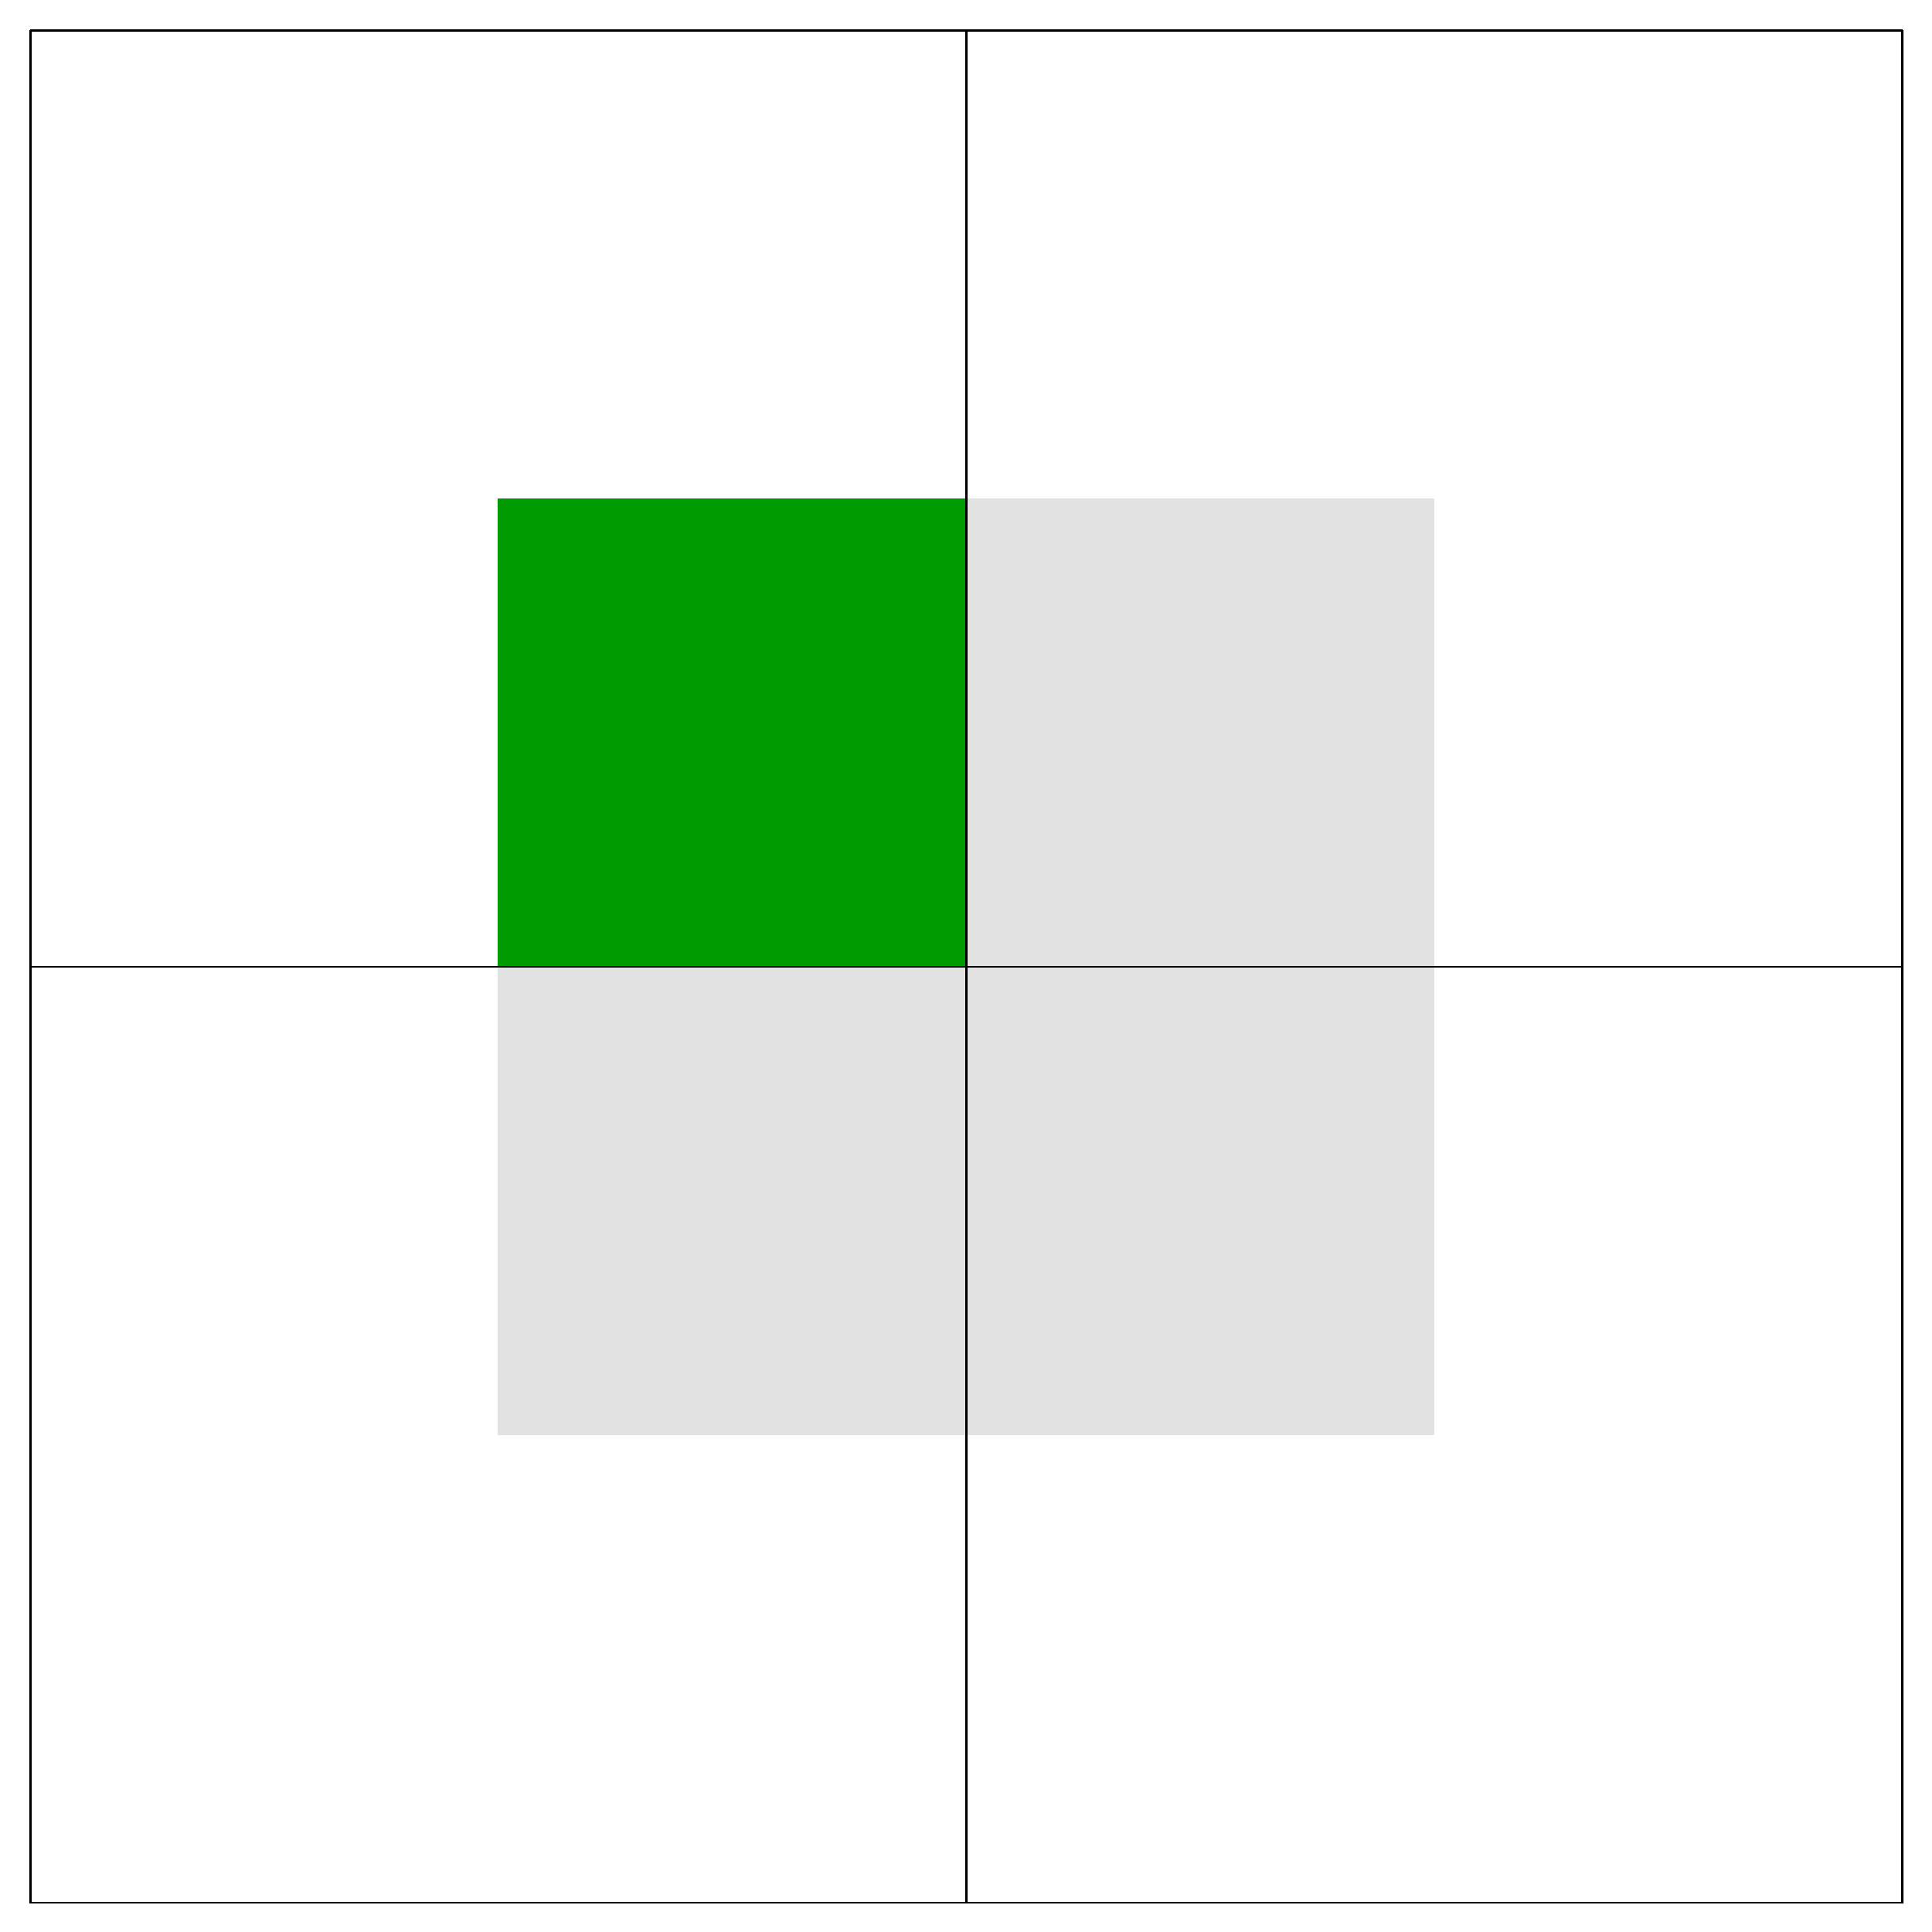
\includegraphics[width=\linewidth]{drawings/cubes_07.pdf}
  Voxel 7
\endminipage
\minipage{0.25\textwidth}%
  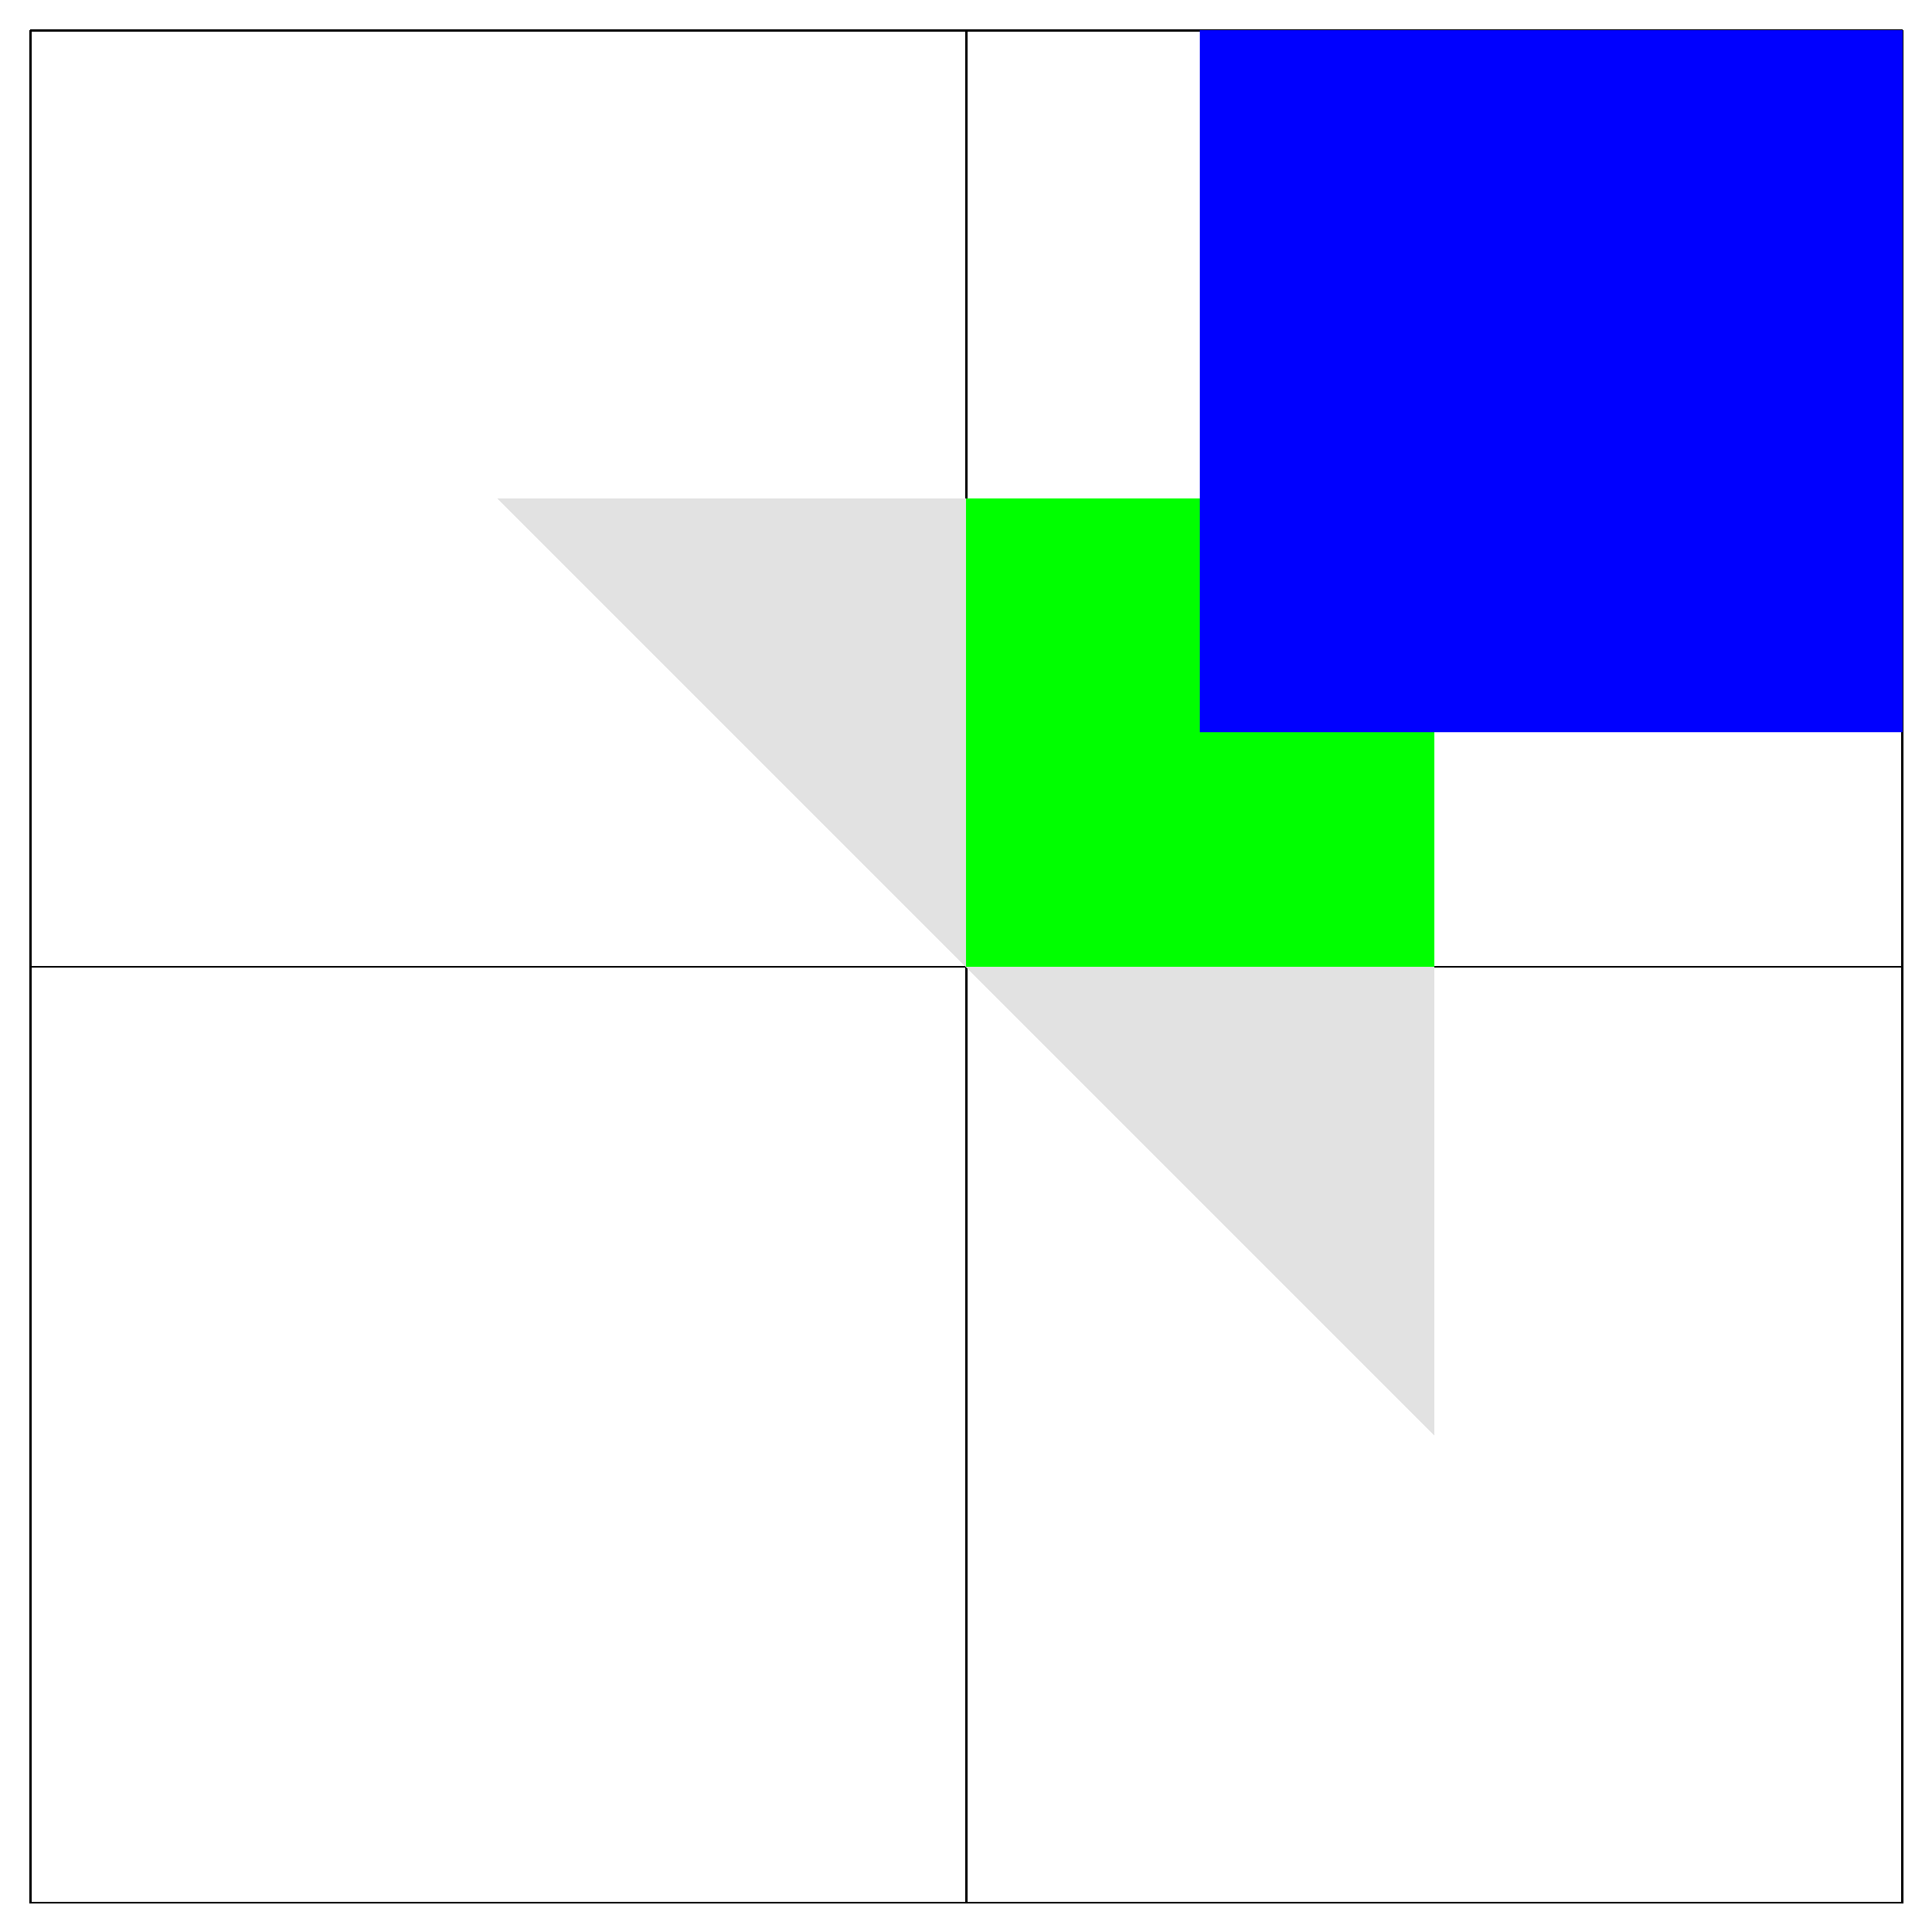
\includegraphics[width=\linewidth]{drawings/cubes_04.pdf}
  Voxel 4
  
  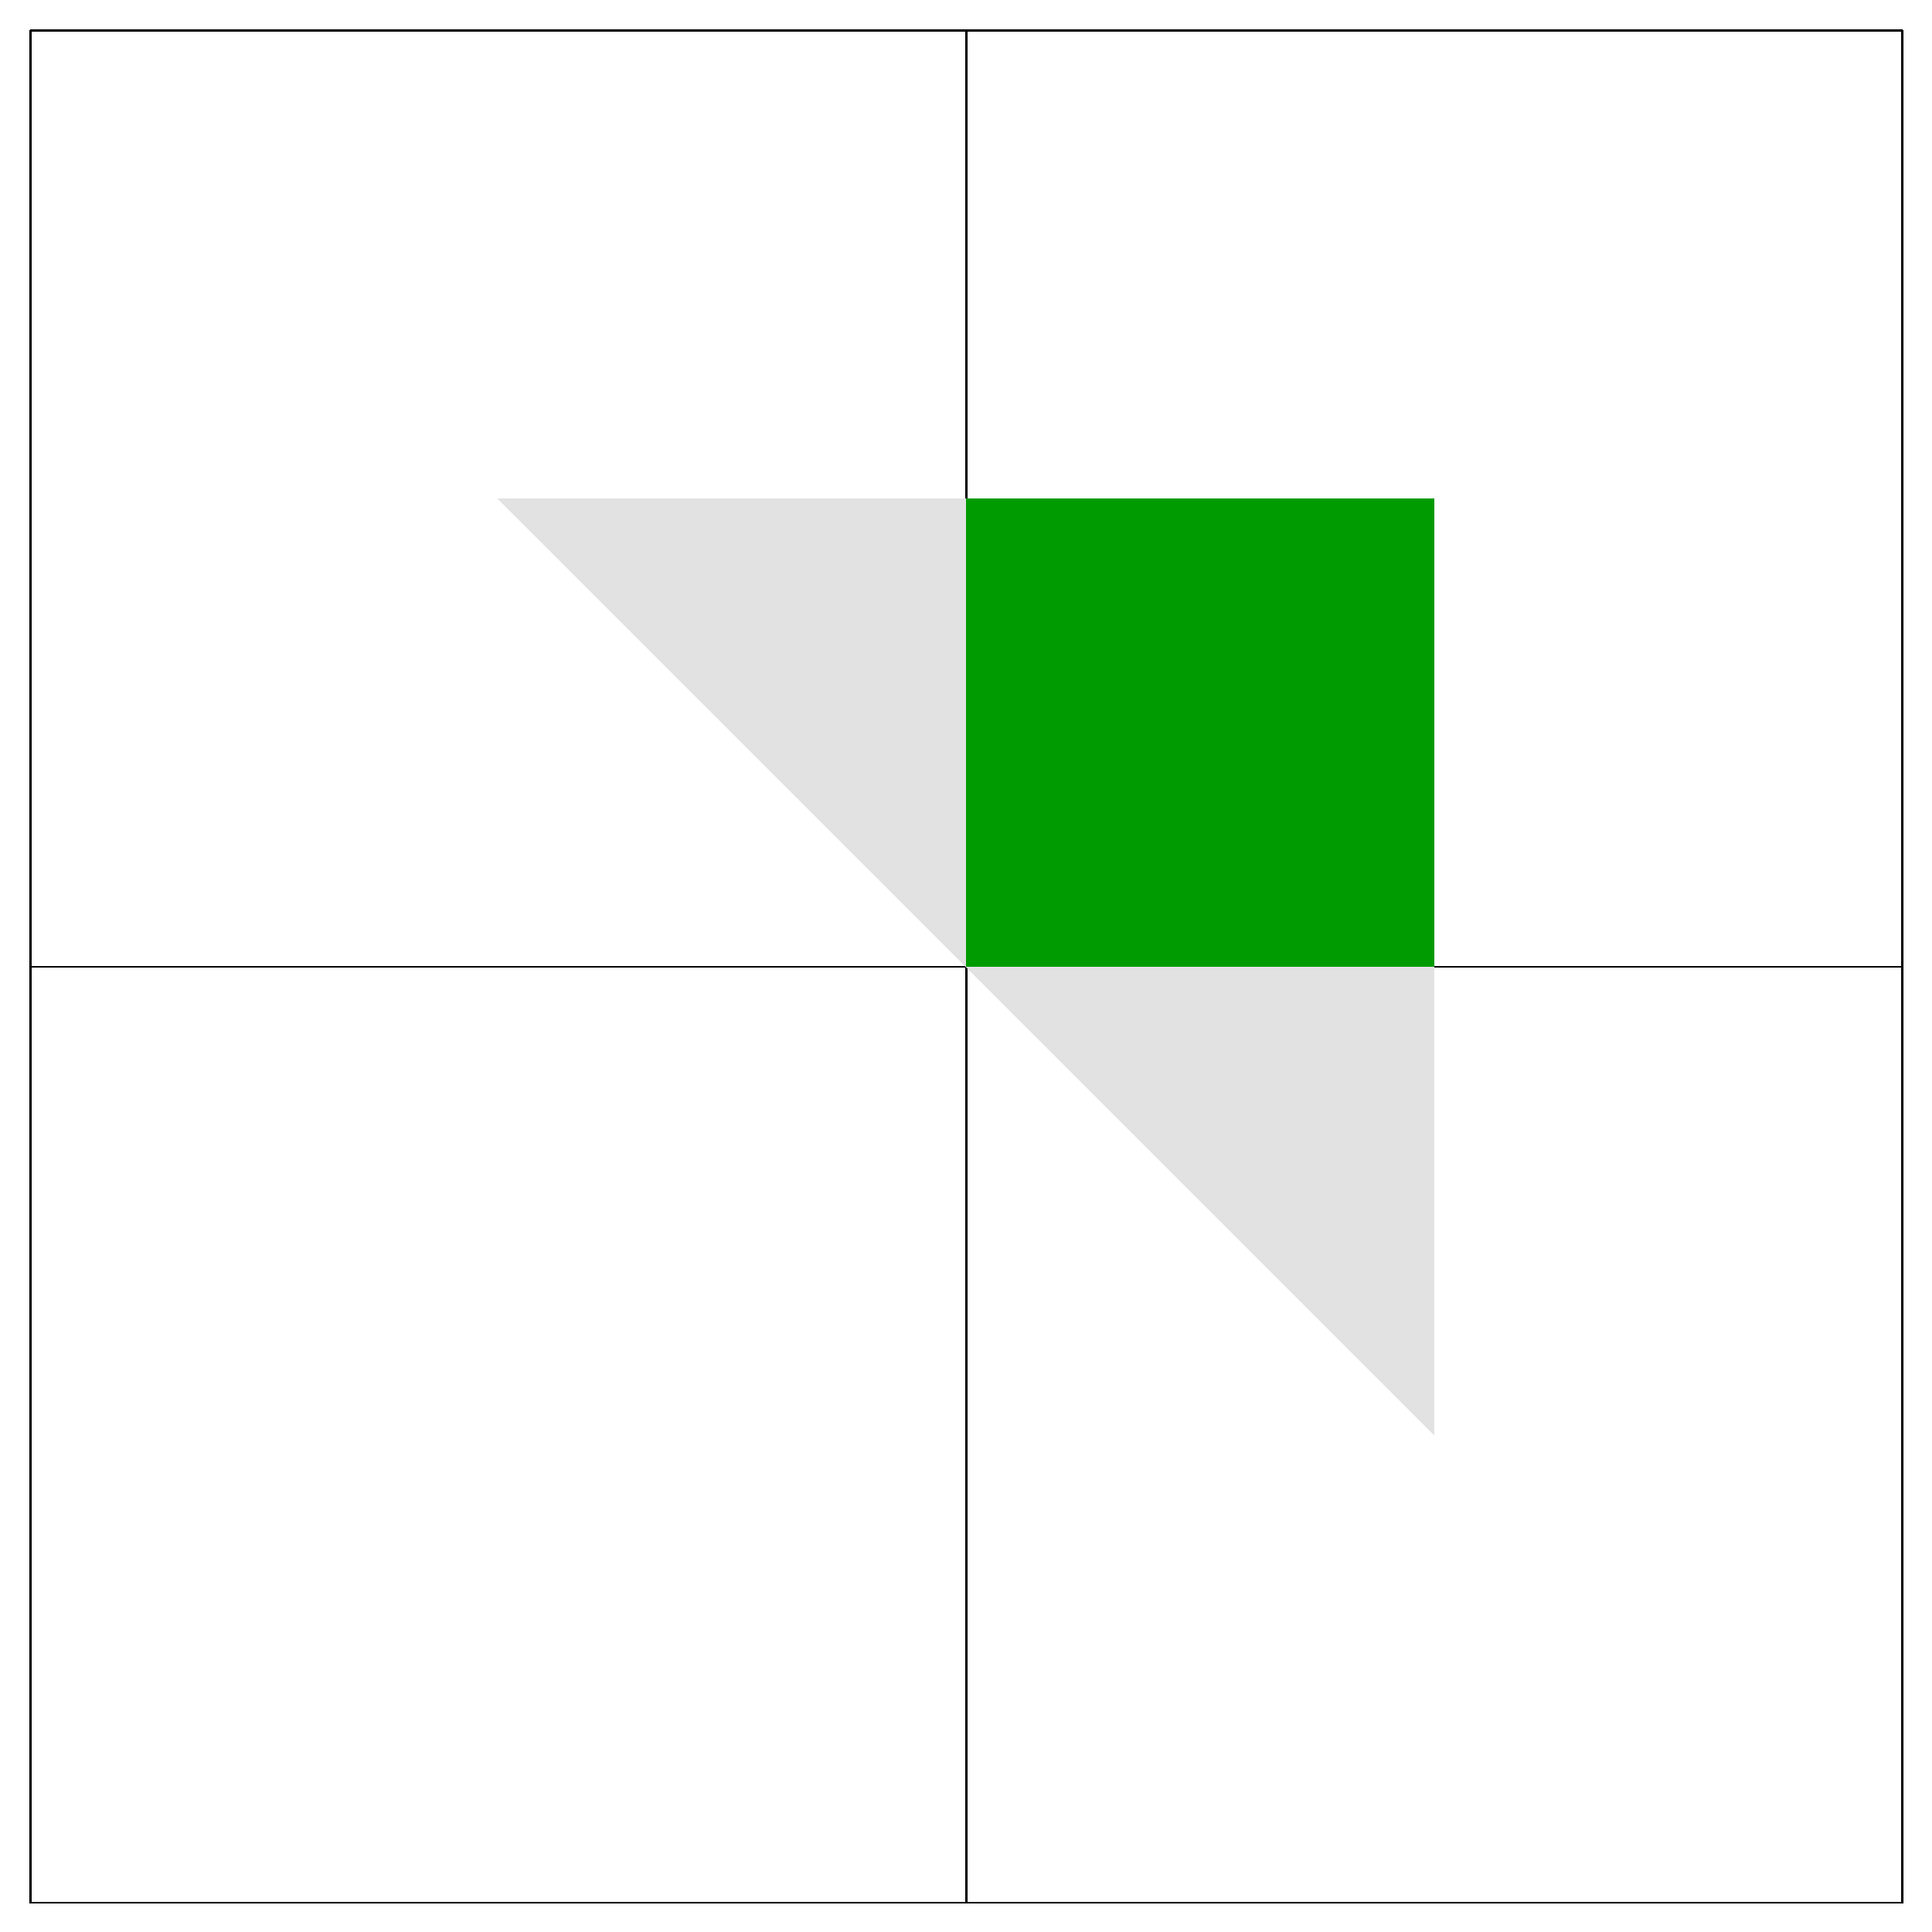
\includegraphics[width=\linewidth]{drawings/cubes_08.pdf}
  Voxel 8
\endminipage
\caption{Images produced by each traced voxel}
\label{fig:cubes}
\end{figure}

\begin{figure}[!htb]
\centering
  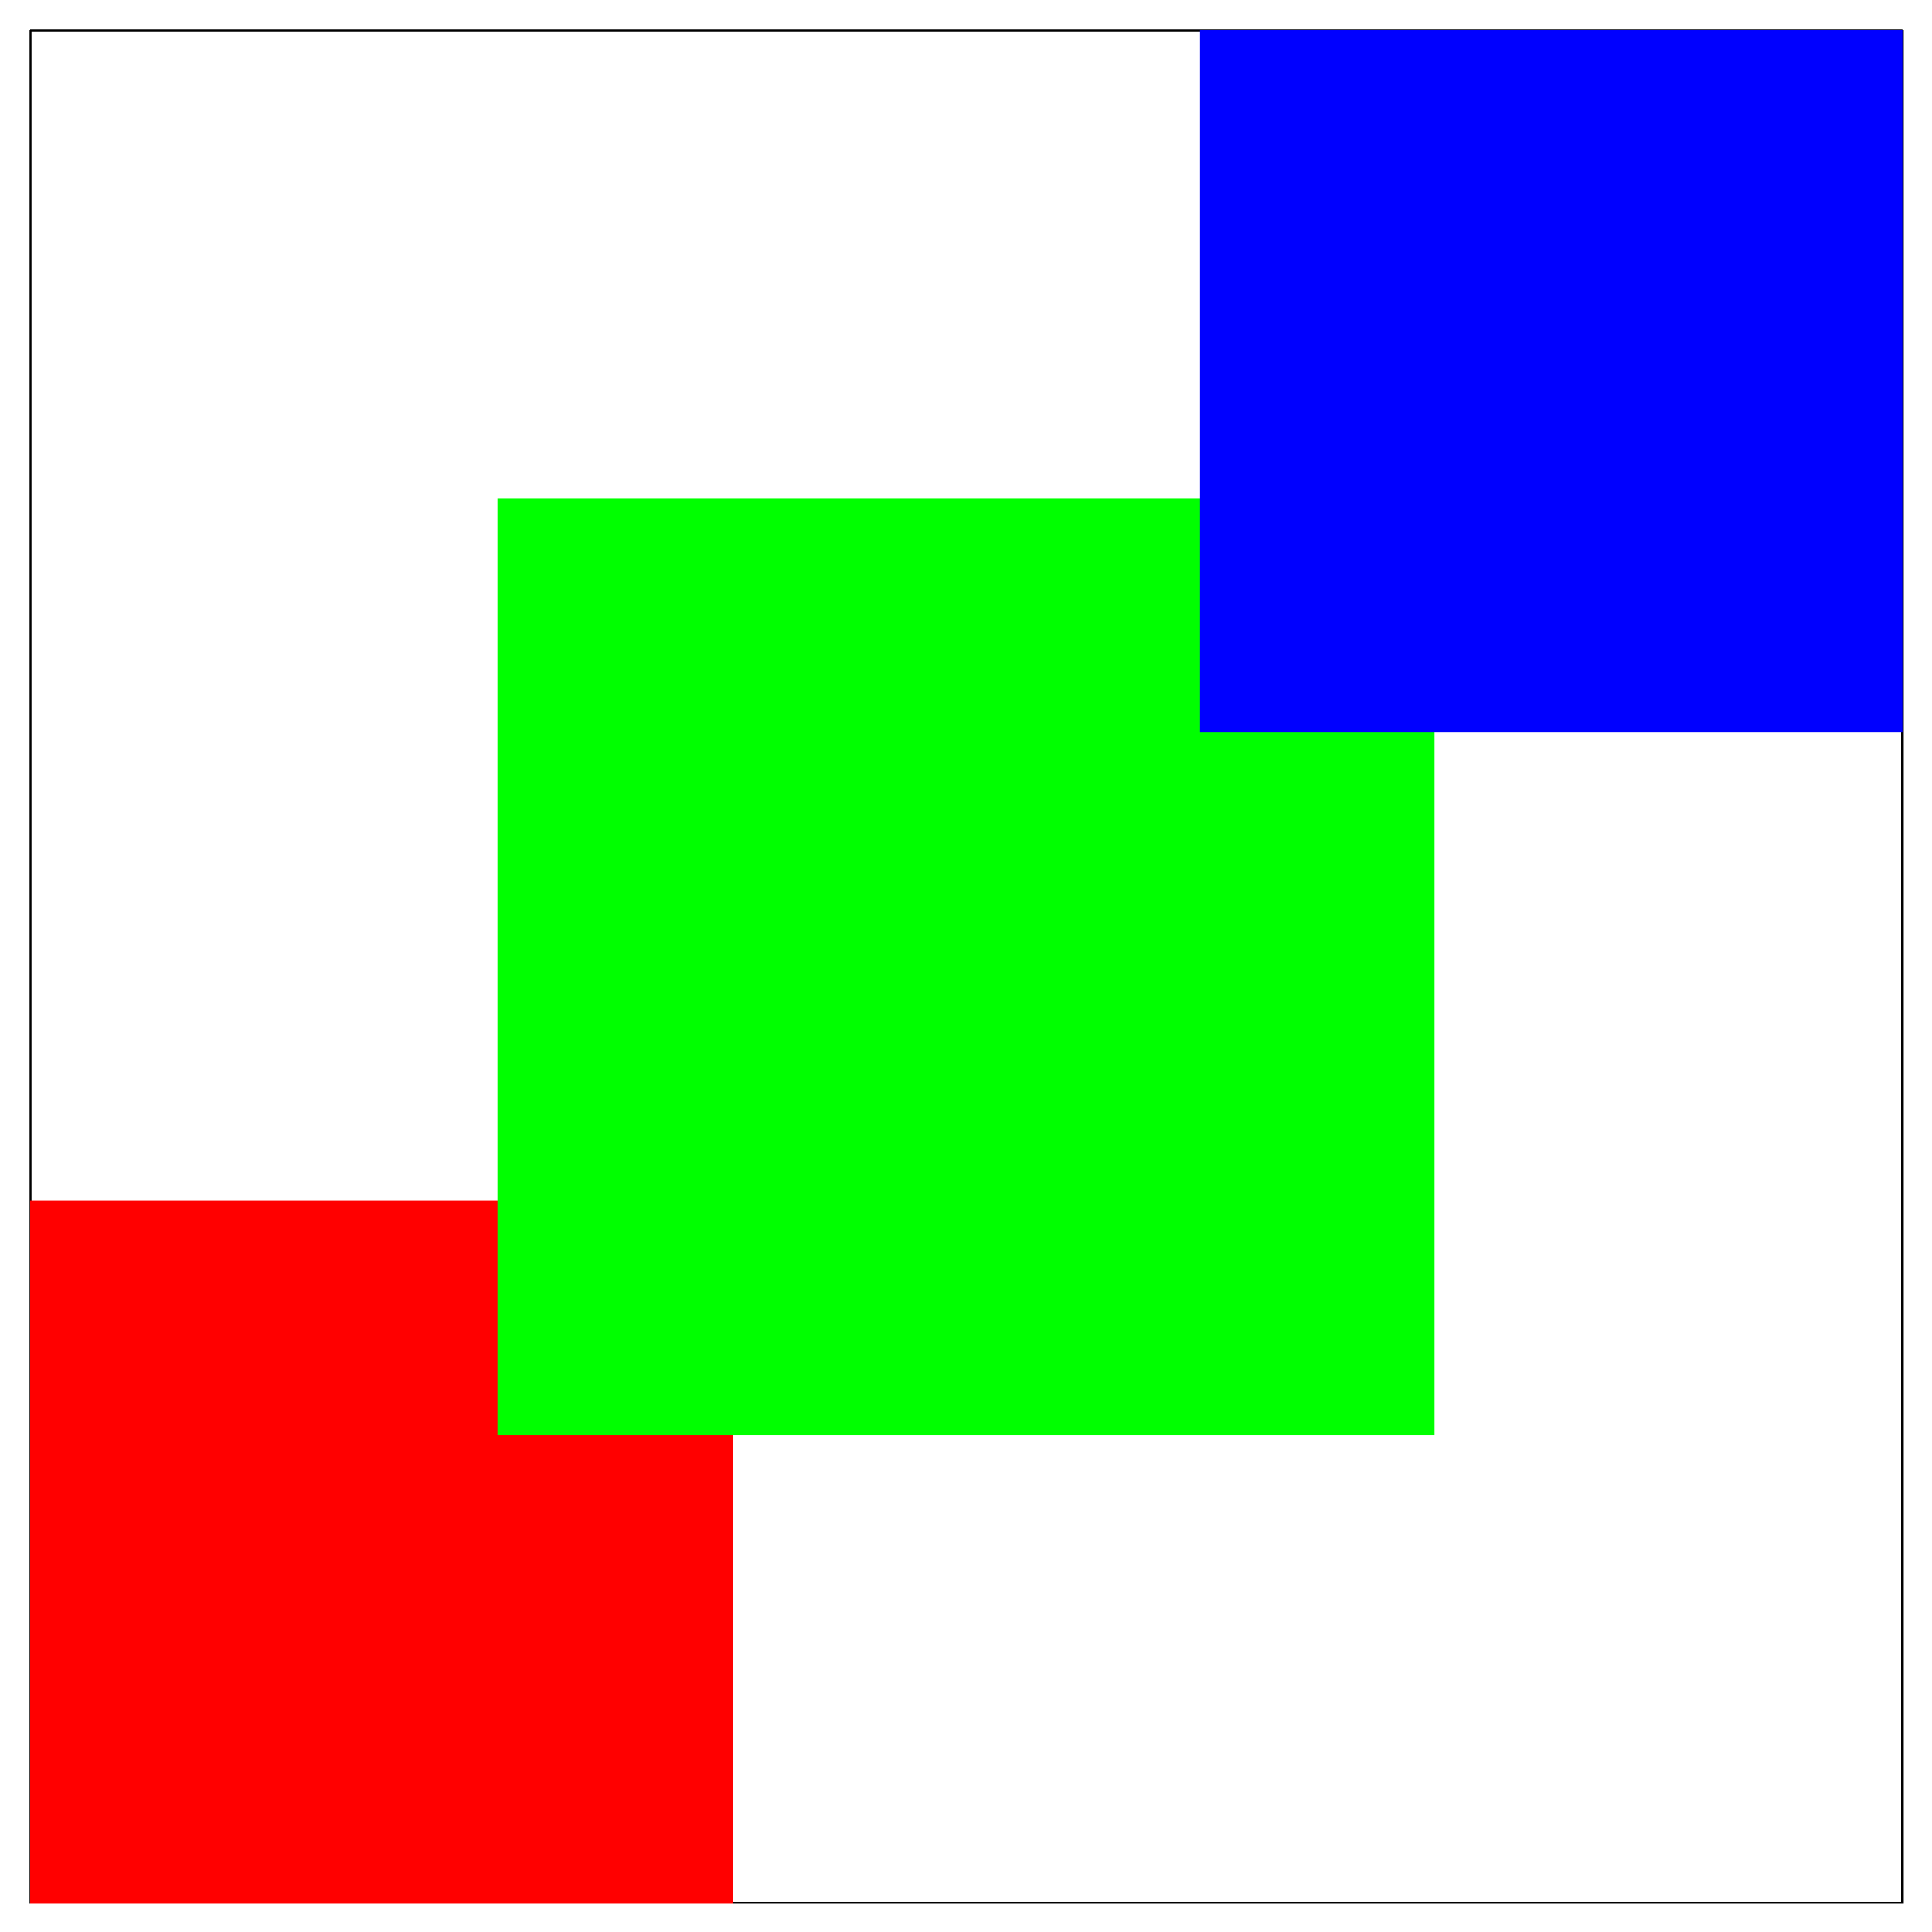
\includegraphics[height=5cm]{drawings/cube_final.pdf}
\caption{Final composed image of traced voxels}
\label{fig:cubes_final}
\end{figure}


\subsection{Communication avoiding ray tracing}
\label{sec:ca-ray-tracing}

Expanding on the ray casting algorithm, we will now look at how we might design 
similar communication avoiding algorithms to implement a full ray tracer.  We 
will first tackle secondary light rays, these are rays cast from an intersection
point to a light source.  To correctly compute shadows, it is important to know 
if the ray intersects with any other objects in the scene anywhere along its 
path from the intersection point of the object to the light source.  

Shadow ray calculations could result in a significant amount of communication if
done during runtime.  To reduce this cost, we introduce a technique that 
distributes light information to each voxel prior to runtime.  Similar to the 
ray casting algorithm, we can cast rays into the scene from each light source.  
Instead of sending all rays to all voxels however, we will need to propagate the
rays through the scene, starting with the light source and moving outward.  As
the rays are propagated they can be marked as in shadow or not.  As the light
rays reach a new voxel, they produce a mesh on the facing wall.  Each vertex in
the mesh then would contain either an indicator that the vertex is in shadow or
the direction and illumination information from its light source, see 
figure~\ref{fig:light-distribution}.  Additional information on 
implementation can be found in section~\ref{sec:proposed_algorithm}.

\begin{figure}[!htb]
\centering
\begin{subfigure}{0.49\textwidth}
 \centering
  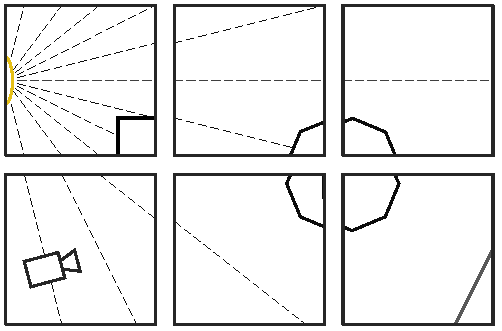
\includegraphics[width=.98\columnwidth]{drawings/Lights1.pdf}
  \caption{Initial light rays}
\end{subfigure}
\begin{subfigure}{0.49\textwidth}
 \centering
  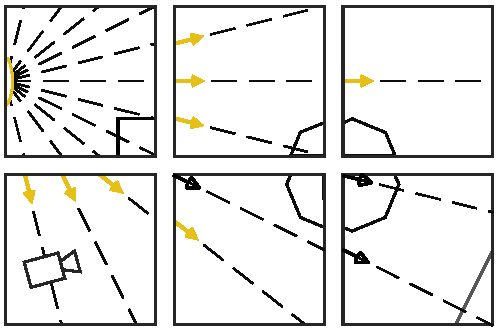
\includegraphics[width=.98\columnwidth]{drawings/Lights2.pdf}
  \caption{Computed light mesh}
\end{subfigure}
\caption{Light ray distribution}
\label{fig:light-distribution}
\end{figure}

The computed light is then used at runtime by the voxel computation to 
compute secondary light rays without needing to communicate with any other 
voxel.  The individual voxel, using the location of each light source can 
compute rays from an intersection point to each light source.  At the 
intersection of the ray to a voxel wall, the corresponding light mesh will be 
used to determine the correct illumination necessary for the intersection point.
A nearest neighbor or averaging algorithm can be used to determine which vertex 
in the mesh is closest to the intersection point.  The information from the 
selected vertex or vertices can then be used for the illumination calculation.

\subsubsection{Reflected and refracted rays}
Although not implemented within the scope of this thesis, we introduce a 
potential communication avoiding strategy for handling reflected and refracted 
rays.  For refracted rays, a technique similar to the light meshes could be 
used, where a mesh is computed from each reflected material and distributed 
outward to each voxel.  Instead of holding light and shadow information the 
vertices of the mesh would contain material information from the first object 
intersected.  Each voxel computation would then use the material mesh to 
determine the correct color for a reflected ray.  Each voxel would need access 
to all the material meshes in the case where a reflected ray reflects to another
reflector.  See section~\ref{sec:future-work} for additional details.

Refractor materials which change the trajectory of the rays that pass through 
them could be supported by the proposed algorithm through the use of a restart 
capability.  The underlying assumptions to compute the light and material meshes
rely on the rays maintaining a straight trajectory.  The same assumption is made
to compute the intersection of the primary viewing rays and each voxel they
intersect with.  If a ray refracts in one voxel, the subsequent voxels would
need to know the new intersection point of that ray and their wall, along with
the rays new direction.  If we could detect when rays refract within a voxel and
invalidate the computations being done with non-refracted rays, we could restart
them with the correct rays.  Details on this technique can be found in 
section~\ref{sec:future-work}.

If a scene contains little or no reflected rays, the overhead of computing the
material meshes may outweigh the cost of communicating reflected rays at 
runtime.  If the material meshes and the light meshes are used however 
communication cost would be reduced to one pass through the domain for each 
light and each reflector prior to runtime.  At runtime each voxel's computation
would be an independent calculation, requiring no communication except to send
back the final results of the traced rays.  The use of meshes however, results 
in an approximation of the result produced by a conventional ray tracer due to 
the nearest neighbor or averaging used when a ray intersects the mesh.

\section{Proposed Algorithm}
\label{sec:proposed-algorithm}
Using a spatially even data distribution algorithm as described in 
section~\ref{sec:data_decomposition} and reducing communication as described in 
section~\ref{sec:communication} allows us to design the communication 
avoiding ray tracer outlined in Figure~\ref{fig:design}.  The figure shows a 
Petri Net, see Section~\ref{sec:petri-nets}, describing the main components of 
a full ray tracing algorithm.  The following sections break down each place and
transition.  For the scope of this thesis we have implemented the highlighted 
section, details can be found in chapter ~\ref{sec:implementation}.

\begin{figure}[!htb]
\centering
  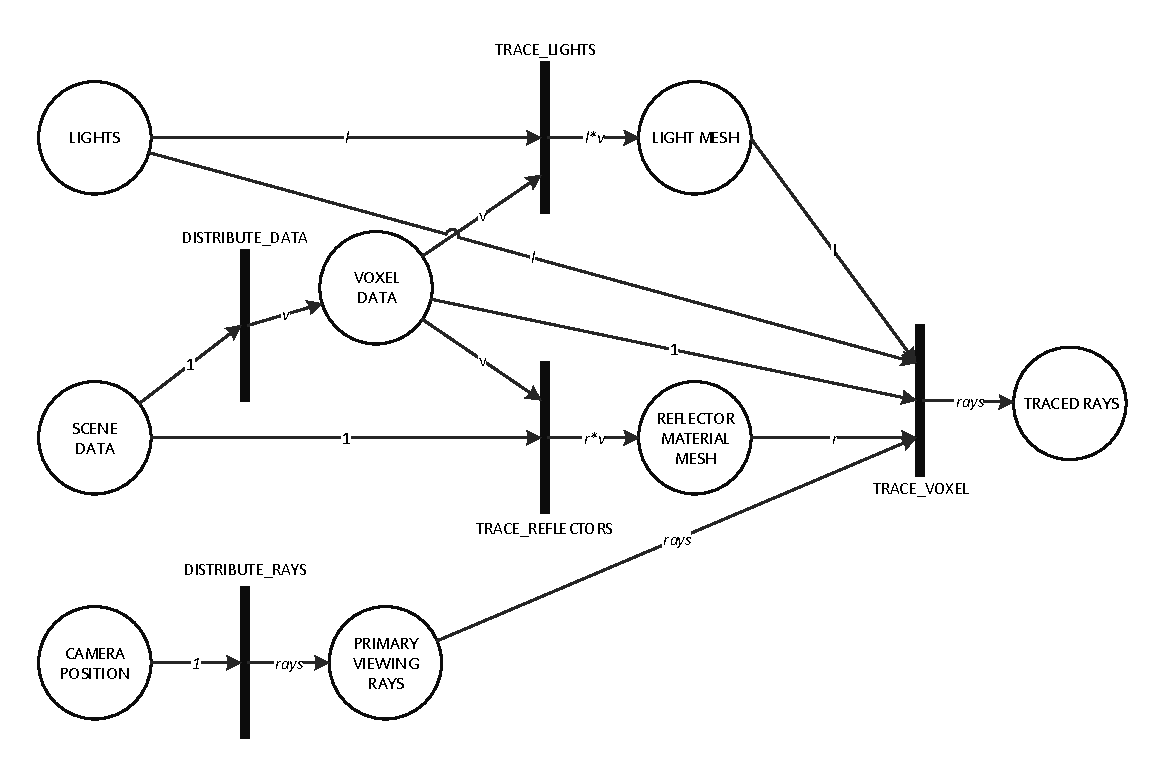
\includegraphics[width=\linewidth]{drawings/Design.pdf}
\caption{Proposed Design Petri Net}
\label{fig:design}
\end{figure}

\subsection{Inputs}
The required inputs for the ray tracer are three places; lights, scene, and 
camera position.  There will be a single scene with potentially many lights.  
Additionally many camera positions can be traced, but each pass through 
\emph{traced rays} will use a single camera position.  The labels on the arcs 
indicate the quantity relationships.

\begin{figure}[!htb]
\minipage{0.4\textwidth}
\begin{algorithm}
DISTRIBUTE_DATA(scene, v)
  in:  the scene to be traced
       number of voxels, v
  out: v subsets of data
  voxels[v]
  for all voxel in voxels do
    for all trangles in scene do
      if trangle is in voxel then
        voxel.data.add(trangle)
      end if
    end for
  end for
return voxels
\end{algorithm}

Distribute data
\endminipage\hfill
\caption{Ray tracer pseudo code}
\label{fig:ray_tracing_1}
\end{figure}

\subsection{Distribute data}
The transition, \textbf{distribute\_data} takes a scene as an input and produces 
\emph{v} subsets of the data, one for each voxel.  \emph{Voxel Data} contins the
resulting data sets, see Figure~\ref{fig:ray_tracing_1}.

\subsection{Distribute rays}
The transition, \textbf{distribute\_rays} takes either a camera position as input 
or information regarding refracted rays from the output of a voxel computation 
and produces a set of viewing rays.  \emph{Primary Viewing Rays} are the 
resulting computed sets.

\begin{figure}[!htb]
\minipage{0.4\textwidth}
\begin{algorithm}
TRACE_LIGHTS(lights, voxels) 
  in:  lights in the scene
       voxel data
  out: light mesh for each voxel
  for all light in lights do
    light_mesh = false;
    for all voxel in voxels do 
      if not light_mesh then
        light_mesh = 
          COMPUTE_MESH(light, voxel)
      else
        light_mesh = 
          PROPIGATE_MESH(light_mesh, 
                       light, voxel)
      end if
      light_mesh_ = COPY(light_mesh)
      voxel.light_meshes.add(light_mesh_)
    end for
  end for
return voxels


.
\end{algorithm}

(a) Trace lights

\endminipage\hfill
\minipage{0.4\textwidth}
\begin{algorithm}
TRACE_REFLECTORS(scene, voxels) 
  in:  scene to be traced
       voxel data
  out: material mesh for each reflector
  material_meshes[,]
  for all objects in scene do
    material_mesh = false
    if object is reflector then
      for all voxel in voxels do 
        if not light_mesh then
          material_mesh = 
            COMPUTE_MESH(object, voxel)
        else
          material_mesh = 
            PROPIGATE_MESH(material_mesh, 
                         object, voxel)
        end if
      end for
      material_meshes.add(object, 
                         material_mesh)
    end if
  end for
return material_meshes
\end{algorithm}

(b) Trace reflectors

\endminipage\hfill
\caption{Ray tracer pseudo code}
\label{fig:ray_tracing_2}
\end{figure}

\subsection{Trace lights}
The transition, \textbf{trace\_lights} fires for each light in the domain and
uses the voxel data sets to produce a light mesh for each light for each
voxel.  \emph{Light Mesh} is the resulting mesh.  Pseudo code can be found in 
Figure~\ref{fig:ray_tracing_2} a.

\subsection{Trace reflectors}
The transition, \textbf{trace\_reflectors} fires once for each scene and 
produces a material mesh for every reflector in the scene for each voxel.  
\emph{Reflector Material Mesh} is the resulting mesh.  The pseudo code for trace 
reflectors is similar to the pseudo code for trace lights and is presented in
 Figure~\ref{fig:ray_tracing_2} b.

\subsection{Trace voxel}
The transition, \textbf{trace\_voxel} fires once for each voxel and produces a 
copy of the viewing rays with computed color information.  \emph{Traced Rays} 
are the resulting rays.  This transition uses the light meshes created for 
its voxel along with the material meshes.  It will also need the primary viewing 
rays and the lights.  Pseudo code for trace voxel can be found in 
Figure~\ref{fig:ray_caster}.  Pseudo code for the helper method 
\textbf{compute\_color} is included in Section~\ref{sec:implementation}.


\begin{figure}[!htb]
\minipage{0.45\textwidth}
  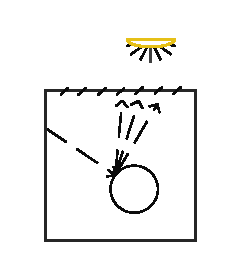
\includegraphics[width=6cm]{drawings/Case_1.pdf}
  
  (a) Light rays with no obstruction; handled by light mesh
  
  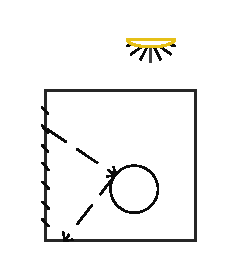
\includegraphics[width=6cm]{drawings/Case_3.pdf}
  
  (c) Reflected rays; handled by material mesh
  
\endminipage\hfill
\minipage{0.45\textwidth}
  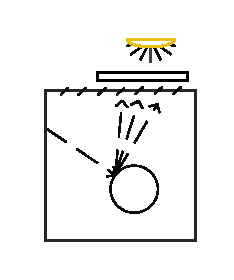
\includegraphics[width=6cm]{drawings/Case_2.pdf}
  
  (b) Light rays with obstruction; handled by light mesh
  
  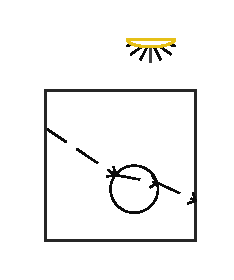
\includegraphics[width=6cm]{drawings/Case_4.pdf}
  
  (d) Refracted rays; handled by restart
  
\endminipage
\caption{Ray tracing algorithm cases}
\label{fig:use-cases}
\end{figure}

The algorithm presented here will handle ray casting as well as ray tracing for
scenes with multiple light sources as well as materials with reflection and
refraction material types.  The light mesh implementation can be found in 
section~\ref{sec:implementation}.  Additional detials on material meshse and the 
restart technique proposed for refracted rays can be found in section
~\ref{sec:future-work}.  A summary of the use cases supported are outlined in
figure~\ref{fig:use-cases}.
















 

\chapter{Implementation}

When designing our ray tracing prototype for exascale we focused on
two key aspects: (a) producing a task based application with (b) an
emphasis on avoiding communication. For simplicity, we consider here
only ray tracing scenes without reflection or refraction, although our
proposed algorithm can be extended to handle either in the future. Our
algorithm uses a simple voxel decomposition to split the work required
to trace a scene (which we will henceforth refer to as a ``domain'').

Primary camera rays are then sent into the system and propagate
through the domain. As secondary rays introduce most of the uncertainty
in the amount of communication necessary in a ray tracing algorithm,
we introduce a pre-processing technique that distributes light
information to each voxel prior to tracing the domain. This allows the
ray tracing step within each voxel to be completely independent of the
data in the rest of the domain. Using this algorithm we can predict an
upper bound on the amount of communication necessary (a domain that
contains no data), and extrapolate from there rough estimates on how
our algorithm might perform on an exascale system.

\section{Implementation}
\label{sec:implementation}

We chose to implement our ray tracer using Intel’s implementation of
CnC, which is built on top of their Thread Building Blocks (TBB)
library. This runs on today’s multicore systems but has the potential
to do so on anticipated exascale systems.

% apparently putting this here makes it show up on the top of page 3, where I want it
\begin{figure}[t]
  \centering
  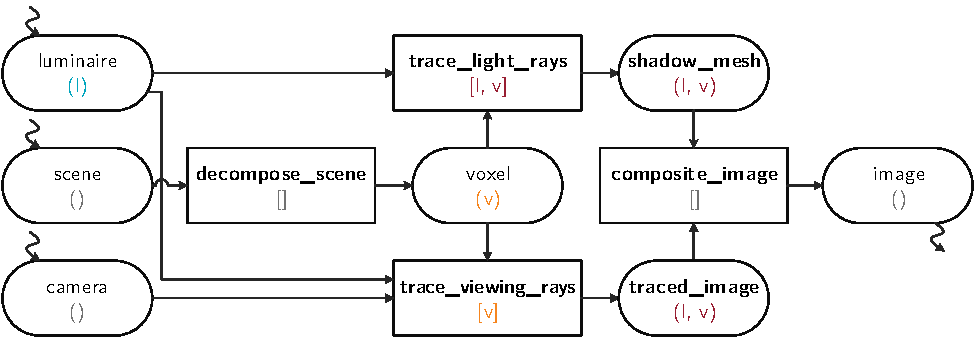
\includegraphics[width=\textwidth]{drawings/CnC.pdf}
  \caption{CnC Graph}
  \label{fig:cnc}
\end{figure}

Figure \ref{fig:cnc} shows the graph for our distributed ray tracer.
It shows data collections, step collections, and the dependencies
between them. The tags corresponding to each collection are also
shown. The control collection for the proposed model is static for all
steps and defined in an initialization step. The graph begins
execution when the object, lights, and camera data are provided, and
terminates when it produces an image.

Let us consider the parts of the graph individually.

\section{Tags}

The tags are different for many of the data and step collections but
share common elements. The FRAME tag refers to one specific frame in
the case of an animation. The INSTANCE tag refers to the current
iteration. The I, J, and K tags are iterators over 3D spatial data,
selecting a specific voxel. The RAY\_STEP tag allows for multiple
traversals of the same voxel in the same frame for secondary rays.

\section{Data Collections}
\label{sec:datacollections}

The OBJECT data collection contains input data for the domain from the
environment. Currently, this data is extracted from WaveFront
``\texttt{.obj}'' files. The DECOMPOSE\_DOMAIN step collection
partitions this data into voxels, producing the VOXEL\_OBJECT data
collection. Objects that span multiple voxels are duplicated. The
LIGHTS data collection contains data pertaining to light sources. The
VOXEL\_LIGHT data collection contains the same information as LIGHTS
plus a traced light mesh for each wall of a voxel. The CAMERA data
collection contains the location and direction of the camera. The
RAY\_PACKET data collection contains all the rays that intersect a
voxel wall for a given wall and iteration. The IMAGE data collection
contains the final image data.

\section{Step Collections}

Recall that these are where the computation is done. They may be
implemented in any programming language CnC supports, which is most of
them.

\subsection{DECOMPOSE\_DOMAIN}

As mentions in Section~\ref{sec:datacollections} the DECOMPOSE\_DOMAIN
step takes the data to be traced as input and produces subsets of that
data based on voxel decomposition. As load balancing is not a concern,
a uniformly-gridded voxel decomposition is sufficient. The number of
voxels produced is set at runtime and should be more than the number
of nodes available.
% RRL: Is this really a constraint?

\subsection{DISTRIBUTE\_LIGHTS}

In order to reduce the communication of secondary rays,
the DISTRIBUTE\_LIGHTS step is responsible for distributing light
information to each voxel. This guarantees each voxel will only need
to communicate with its direct neighbors. The light information
produced for each voxel contains the original light sources as well as
a light source mesh for each light and each wall of the voxel. The
mesh is produced by tracing rays from each light source to uniformly
spaced points along a voxel wall, see Figure \ref{fig:light}. Where
the rays intersect the wall, new point or directional light sources
are created. If the ray is blocked, the node in the light mesh is
tagged as in shadow.

\begin{figure}[!htb]
\centering
\begin{subfigure}{0.49\textwidth}
 \centering
  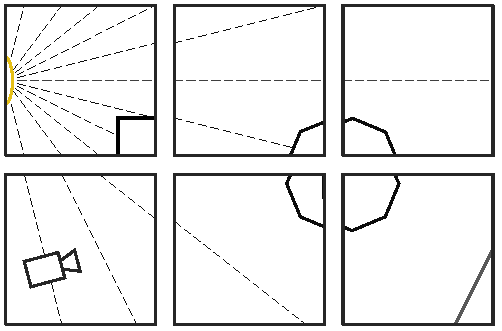
\includegraphics[width=.98\columnwidth]{drawings/Lights1.pdf}
  \caption{Initial light rays}
\end{subfigure}
\begin{subfigure}{0.49\textwidth}
 \centering
  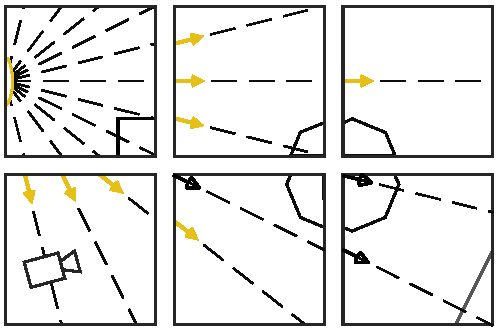
\includegraphics[width=.98\columnwidth]{drawings/Lights2.pdf}
  \caption{Point light sources}
\end{subfigure}
\caption{Light Ray Distribution}
\label{fig:light}
\end{figure}

\subsection{DISTRIBUTE\_RAYS}

The DISTRIBUTE\_RAYS step is responsible for sending each voxel its
first iteration of ray information. This is an empty set of data for
all voxels except the voxel containing the camera if the camera is
positioned within the domain. If the camera is outside the domain
(e.g. in an orthographic view), multiple voxels may be initialized.

\subsection{TRACE\_VOXEL}

The TRACE\_VOXEL step is the heart of the application. This step
executes multiple times for each voxel, depending on the size of the
domain. Each time TRACE\_VOXEL executes, it consumes ray packets from
each of its neighbors. It then traces the rays over its subset of the
domain. If a ray intersects with an object, secondary rays from each
light source are considered if the corresponding point or directional
light source from the voxels light mesh is not in shadow.

Rays that do not intersect objects within the voxels and reach the
voxels walls are collected and passed to the corresponding neighbor on
the next iteration. See Figure~\ref{fig:trace}. Because we are not
considering reflection or refraction, we know the maximum amount of
times we will have to communicate a single ray across voxel borders in
the worst case is proportional to domain size. This allows us to
prescribe the a maximum number of instances of TRACE\_VOXEL in an
initialization step. For the example in Figure~\ref{fig:trace}, that
maximum is 3. As each step will eventually be executed on a single
node of a cluster we plan to implement TRACE\_VOXEL using Embree,
Intel’s ray tracing kernel, in order to optimize per node performance.

\begin{figure}[!htb]
\centering
\begin{subfigure}{.49\columnwidth}
 \centering
  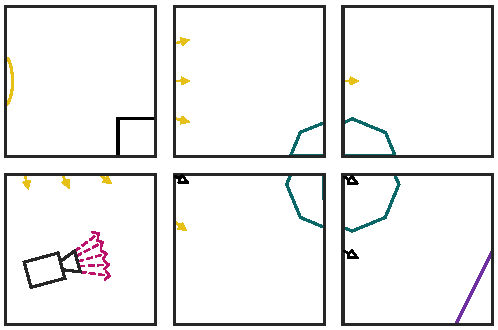
\includegraphics[width=.98\columnwidth]{drawings/Trace1.pdf}
  \caption{Distribute rays}
\end{subfigure}
\begin{subfigure}{.49\columnwidth}
 \centering
  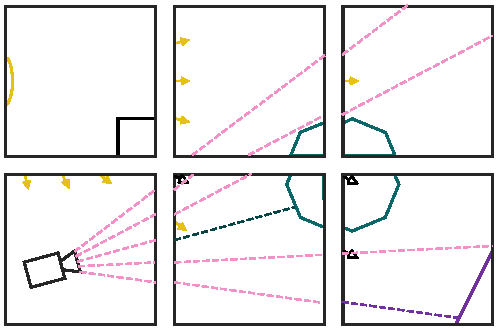
\includegraphics[width=.98\columnwidth]{drawings/Trace2.pdf}
  \caption{Trace voxel; ray step 1}
\end{subfigure}
\begin{subfigure}{.49\columnwidth}
 \centering
  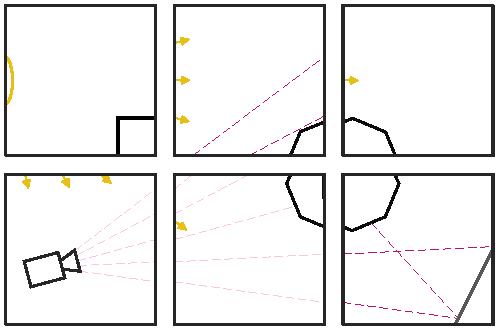
\includegraphics[width=.98\columnwidth]{drawings/Trace3.pdf}
  \caption{Trace voxel; ray step 2}
\end{subfigure}
\begin{subfigure}{.49\columnwidth}
 \centering
  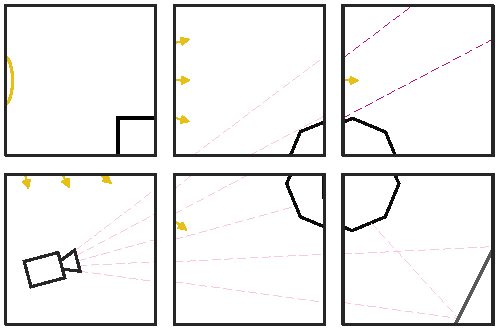
\includegraphics[width=.98\columnwidth]{drawings/Trace4.pdf}
  \caption{Trace voxel; ray step 3}
\end{subfigure}
\caption{Trace Voxel}
\label{fig:trace}
\end{figure}

\subsection{PRODUCE\_IMAGE}
When all steps in TRACE\_VOXEL have completed, the final set of ray
packets is produced. Each ray in that packet contains the information
that may be necessary to produce the final image. Merging these is the
responsibility of the PRODUCE\_IMAGE step.

\section{Textual CnC Graph File}
To give a more concrete example of how the CnC graph file is
implemented, we include a simplified version of the textual
representation of TRACE\_VOXEL in Figure~\ref{fig:tracevoxel}. In
addition to the step declaration, the code includes the SCENE and
RAY\_PACKET data collections as well as the control dependencies from
the environment for TRACE\_VOXEL.

% Code..
\begin{figure*}[t!]
  \begin{center}
    
\begin{lstlisting}[basicstyle=\ttfamily]
/******************************************************************************
//* Item collection declarations */

// data for each voxel, produced by decompose_domain
[ voxel_object *voxel : frame, i, j, k ];

// ray data passed to neighbors, produced by camera and trace_voxel
[ ray_packet *rays : frame, ray_step, neighbor, i, j, k ];

/******************************************************************************
//* CnC steps */

( trace_voxel : frame, ray_step, i, j, k )
<- [ voxel: frame, i, j, k],
   [ rays : frame, ray_step  , 0, i  , j  , k   ] $when(i<#voxels_i-1),
   [ rays : frame, ray_step  , 1, i  , j  , k   ] $when(i>0),
   [ rays : frame, ray_step  , 2, i  , j  , k   ] $when(j<#voxels_j-1),
   [ rays : frame, ray_step  , 3, i  , j  , k   ] $when(j>0),
   [ rays : frame, ray_step  , 4, i  , j  , k   ] $when(k<#voxels_k-1),
   [ rays : frame, ray_step  , 5, i  , j  , k   ] $when(k>0)
-> [ rays : frame, ray_step+1, 0, i-1, j  , k   ] $when(i>0),
   [ rays : frame, ray_step+1, 1, i+1, j  , k   ] $when(i<#voxels_i-1),
   [ rays : frame, ray_step+1, 2, i  , j-1, k   ] $when(j>0),
   [ rays : frame, ray_step+1, 3, i  , j+1, k   ] $when(j<#voxels_j-1),
   [ rays : frame, ray_step+1, 4, i  , j  , k-1 ] $when(k>0),
   [ rays : frame, ray_step+1, 5, i  , j  , k+1 ] $when(k<#voxels_k-1);

/******************************************************************************
//* Input output relationships from environment */

( $initialize: () )
-> (trace_voxel : $range(0, #num_frames), $range(0, #ray_steps),
           $range(0, #voxels_i), $range(0, #voxels_j), $range(0, #voxels_k));

\end{lstlisting} 
  \end{center}
  
  \caption{The TRACE\_VOXEL Section of the CnC Graph File. This has
    been somewhat simplified for readability.}
  \label{fig:tracevoxel}
\end{figure*}

Under the \emph{Item collection declaration} section we see two item
collections being declared. Once for the domain and one for the ray
packets. Instances of the domain indexed using frame, i, j, and k
which correspond to the frame in the case of an animation and the
3-dimensional identifier for a given voxel. Ray packets are indexed
similarly but also include an entry for the current ray step as well
as a neighbor identifier.

Under \emph{CnC steps} we see the declaration for TRACE\_VOXEL. Each
TRACE\_VOXEL step is indexed using the frame, the voxels i, j, k and
the current ray step. The specific instances of the domain and ray
data consumed and produced by TRACE\_VOXEL can be declared using the
RAY\_STEP tag. The step will always consume its scene data. It may
then consume an incoming ray packet and/or produce an outgoing ray
packet for each of the voxel's interior walls.

Under \emph{Input output relationships from environment} we see the
control for TRACE\_VOXEL. In the initialize step we will produce an
instance of TRACE\_VOXEL for every frame in our animation, for every
step in our ray steps, and for each voxel in our scene's
decomposition.

  
\chapter{Evaluation}
\label{sec:example}

Although purely theoretical, we can walk through a potential execution
of our algorithm and draw some conclusions on how it may perform.
Using the San Miguel data set
% RRL: citation?
and assuming we decompose the domain into 27 equal parts, we get the
distribution shown in Figure~\ref{fig:decomposition}. This will be the
cost of communicating the initial datasets to the nodes where
execution will take place. We will incur these costs again if data
needs to be moved once the algorithm starts executing.

\begin{figure}[!htb]
  \centering
  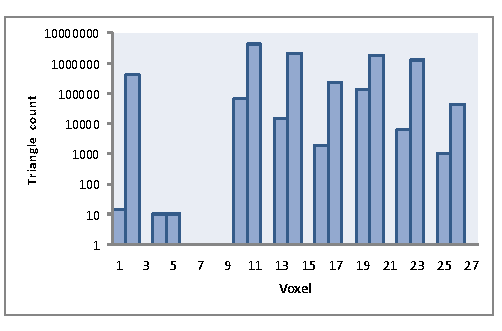
\includegraphics[width=0.5\textwidth]{drawings/DataDistribution.pdf}
  \caption{San Miguel Data Decomposition}
  \label{fig:decomposition}
\end{figure}

If we consider a machine with 8 cores, we might hope to get a distribution 
such as that shown in Figure~\ref{fig:machines}.   This roughly distributes
the data evenly putting an emphasis on positioning neighbors on the same cores.  
Depending on the lights in the scene, we also have to consider the cost of 
distributing them, building the light mesh, and sending the light mesh data 
to each node.  For this example I am assuming the costs associated with the 
lighting is negligible next to the cost of distributed the data in the scene. 

>>> RESUME

\begin{figure}[!htb]
  \centering
  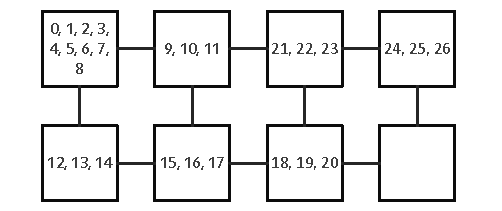
\includegraphics[width=0.5\textwidth]{drawings/NodeDistribution.pdf}
  \caption{Sample Data Distribution}
  \label{fig:machines}
\end{figure} 

Once the algorithm begins execution we can assume a worst case of 3 ray steps being necessary to trace rays from the camera through the scene.  This means each voxel will need to communicate with its neighbors a maximum of 3 times. Some of this communication will be within a node, some will be between nodes.  The cost of this communication needs to be factored into our estimates for total time to trace a given scene.  Acquiring accurate estimates for this equation will be the focus of our future work as exascale systems do not yet exist.  


\chapter{Conclusions}
\section{Conclusion}
\label{sec:conclusion}

We have taken the first steps in designing and implementing a ray tracing
algorithm for exascale.  Although we do not have exascale hardware yet, we have 
executed our implementation on today's systems, integrating the task-based 
library, CnC, with the ray tracing kernel library, Embree.  Our ray tracer does
not support all features of common ray tracers, we believe it provides a basis
that can be extended in future work.  We have shown the viability of a
communication-avoiding ray tracer and look forward to exploring aspects of
exascale such as hybrid systems to examine how they may impact our design.


%\chapter{Future Work}
\section{Future Work}
\label{sec:future-work}

\newpage
\singlespacing
\bibliographystyle{plain}
\bibliography{bibliography}

\appendix
% If you really *must* include source code.
% \chapter{Source Code}
% \begin{figure}[!htb]
  \begin{center}
    
\begin{algorithm}
/******************************************************************************
// * CnC Ray Tracer
// *
// * Author: Ellen Porter (ellen.porter@wsu.edu)
// *         Washington State University
// *
//****************************************************************************/

/******************************************************************************
// * Graph parameters */
$context {
  int voxels_i;   // decomposed domain size
  int voxels_j;
  int voxels_k;
  int num_frames; // frames to trace
};

/******************************************************************************
//* Item collection declarations */
//object data for each voxel, produced by decompose_domain
[ voxel_object *object_data : frame, i, j, k ];
// light data for each voxel, produced by distribute_lights
[ voxel_light *light_data : frame, i, j, k ];
// ray data passed to voxels, produced by distribute_rays
[ rays *primary_rays : frame ];
// ray data produced by trace_voxel
[ rays *traced_rays : frame, i, j, k ];

/******************************************************************************
//* CnC steps */
( decompose_domain : frame )
-> [ object_data : frame, 
     $range(0, #voxels_i), $range(0, #voxels_j), $range(0, #voxels_k) ];
( distribute_lights : frame )
<- [ object_data : frame, 
     $range(0, #voxels_i), $range(0, #voxels_j), $range(0, #voxels_k) ]
-> [ light_data : frame, 
    $range(0, #voxels_i), $range(0, #voxels_j), $range(0, #voxels_k) ];
( distribute_rays : frame )
-> [ primary_rays : frame ];
( trace_voxel : frame, i, j, k )
<- [ object_data  : frame, i, j, k],
   [ light_data   : frame, i, j, k],
   [ primary_rays : frame ]
-> [ traced_rays  : frame, i, j, k];
(compose_image : frame )
<- [ traced_rays : frame, 
     $range(0, #voxels_i), $range(0, #voxels_j), $range(0, #voxels_k)];

/******************************************************************************
//* Input output relationships from environment */
( $initialize: () )
-> (decompose_domain : $range(0, #num_frames)),
   (distribute_rays  : $range(0, #num_frames)),
   (trace_voxel      : $range(0, #num_frames), 
       $range(0, #voxels_i), $range(0, #voxels_j), $range(0, #voxels_k)),
   (compose_image    : $range(0, #num_frames));
( $finalize: () );

\end{algorithm} 
  \end{center}
  \caption{Textual CnC graph file}
  \label{fig:cnc-graph-text}
\end{figure}



\end{document}
